\chapter{Introduction}
\label{chap:introduction}
%In the Introduction chapter, I will discuss the current state of medical care for CHF patients. I will present the relevant statistics about hospitalization and mortality. I will then cover the topic of engaging patients in their own self-care, citing relevant studies and statistics. Then finally indicate my proposed solution.


\begin{figure}[H]

	\begin{center}
		\label{fig:WhippedSystem}
		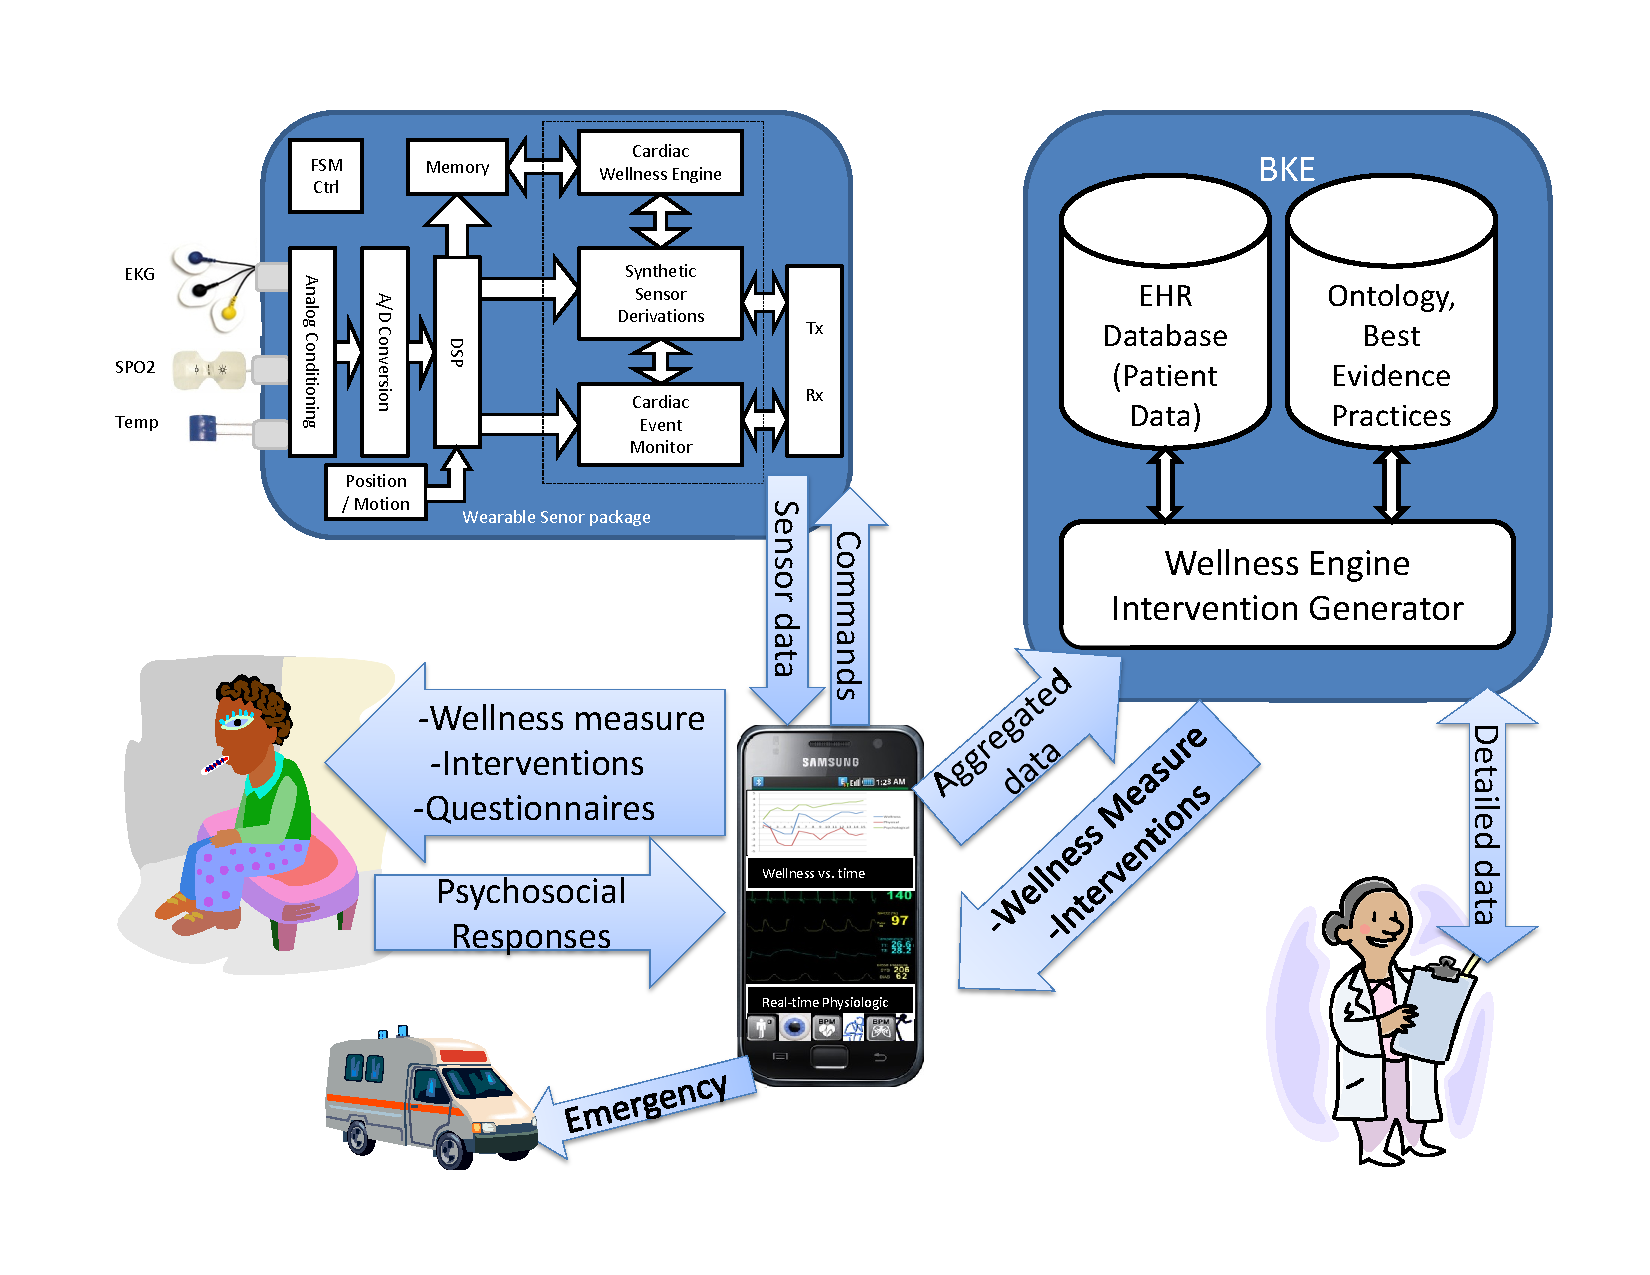
\includegraphics[scale=1,width=0.8  \textwidth]{Images/SystemConcept1.pdf} 
		\caption{WHIPPED System Design}
	\end{center}
\end{figure}

In \Cref{fig:WhippedSystem} we present a new and novel approach to chronic heart failure (CHF) outpatient care called the Wireless Health Indicator Patch for Patient Education and Diagnostics (WHIPPED). CHF is a complex malady caused by numerous disorders of the heart and body resulting in a decreased quality of life (QOL). Care for current cardiac patients, post-hospitalization, is not uniform often resulting in relapses and early death. Despite the emergence of numerous therapeutic innovations, to prolong life and shorten hospital stays, CHF patients often have poor prognosis. Monitoring and involving the patient in self-care can improve upon the prognosis.

This dissertation proposes a new and novel system for cardiac heart failure patient's self-care.  Self-Care encourages an individual to engage in healthy behaviors using targeted educational content. The WHIPPED system  wirelessly collects both physiologic and psychosocial data from the patient using a combination of a custom sensor suite and a smartphone. The collected data is sent to a back-end knowledge engine (BKE) and a wellness measure is calculated by the BKE. Both patient and clinician can access the wellness-score as well as wellness-history. The clinician can, in addition, view the raw data collected by the sensor suite and smartphone. The BKE also analyzes the collected data and offer interventions to patient whose wellness is not improving; reminding a patient to reduce salt or to increase activity levels, for example. Clinicians are also able to interact with the patient if needed. Both types of interactions are available through the patient's smartphone. Lastly, the system can contact emergency services if the patient is suffering from an exacerbation of a cardiac event.  

The WHIPPED system is split into three parts: an integrated mobile sensor platform (WHIP), a smartphone application, and a BKE. A wearable sensor patch collects physiologic readings from the patient using a combination of real and synthetically derived sensors and transmit them to the cell-phone. The cell-phone is used to prompt the patient to answer questions in order to gather psychosocial and symptom data concerning the perceived state of the patient, and send all aggregated data to the BKE. The BKE analyzes the biometric and psychosocial data and calculate a wellness measure for the patient as well as possible interventions designed to improve the patient's wellness and send the results to the smartphone to be displayed to the patient. Furthermore, a clinician can “drill-down” into the raw sensor data to provide additional feedback to the patient. Finally, if an extreme condition or event is detected the system can contact emergency services without the need for patient intervention. 

The WHIP obtains real-time biometric data and wirelessly transmits the metrics for analysis. Using a combination of non-invasive sensors the gathered data is fused to calculate synthetic sensor measurements traditionally requiring additional hardware, moving parts, or devices implanted into the body. The sensor device is designed for long-term use, approximately 30-60 days.

Furthermore, using a smartphone, psychosocial and symptom data is also collected and transmitted for further analysis. The smartphone is also be responsible for communicating the patient's calculated wellness score, clinician's instructions, as well as generated interventions, designed to correct a downward trend in the patient's wellness.  Based on assessed parameters, the patient can receive a message from the system to engage in a health promoting behavior. If a downward trend is detected an intervention is provided to the patient automatically based on the patient's status, co-morbidities, and other factors to attempt to reverse the trend. Finally, the smartphone can contact emergency services in the event of a cardiac event.

The final piece of the implementation, the BKE, computes and tracks the wellness of a patient's heart health over time. The wellness-engine concept is based on prior group research results \cite{Chaiyasucheeva2012} and allows for constant monitoring of a patient's status as well as generating interventions by consulting a modified cardiac ontology also developed by the research group.

Involving the patient in their own self-care can increase their QOL and reduce re-hospitalization. Educating the patient about their illness and care options promotes better decision making when confronted with symptoms.  Self-care is defined as a rational process, involving purposeful choices and behaviors, reflecting knowledge and thought \cite{Riegel2008}. Riegel divides self-care into two concepts, self-care-maintenance and self-care-management.  Self-care-maintenance involves patient monitoring and adherence to a treatment regimen.  In addition, five stages of self-care management are described in \cref{fig:SelfCare}\cite{Riegel2008}. The stages are:
\begin{itemize}
\item  Recognizing and evaluating a status change, 
\item  Deciding an action is needed, 
\item  Taking action, 
\item  Evaluating the effects of the action
\end{itemize}
 Allowing remote monitoring of physiologic and symptom data and providing assisted decision support reduce the burden on medical professionals involved in the care of target patients. Using the WHIPPED system, overall, patient care can be improved and costs can be decreased. 

\begin{figure}[h]
	\begin{center}
		\label{fig:SelfCare}
		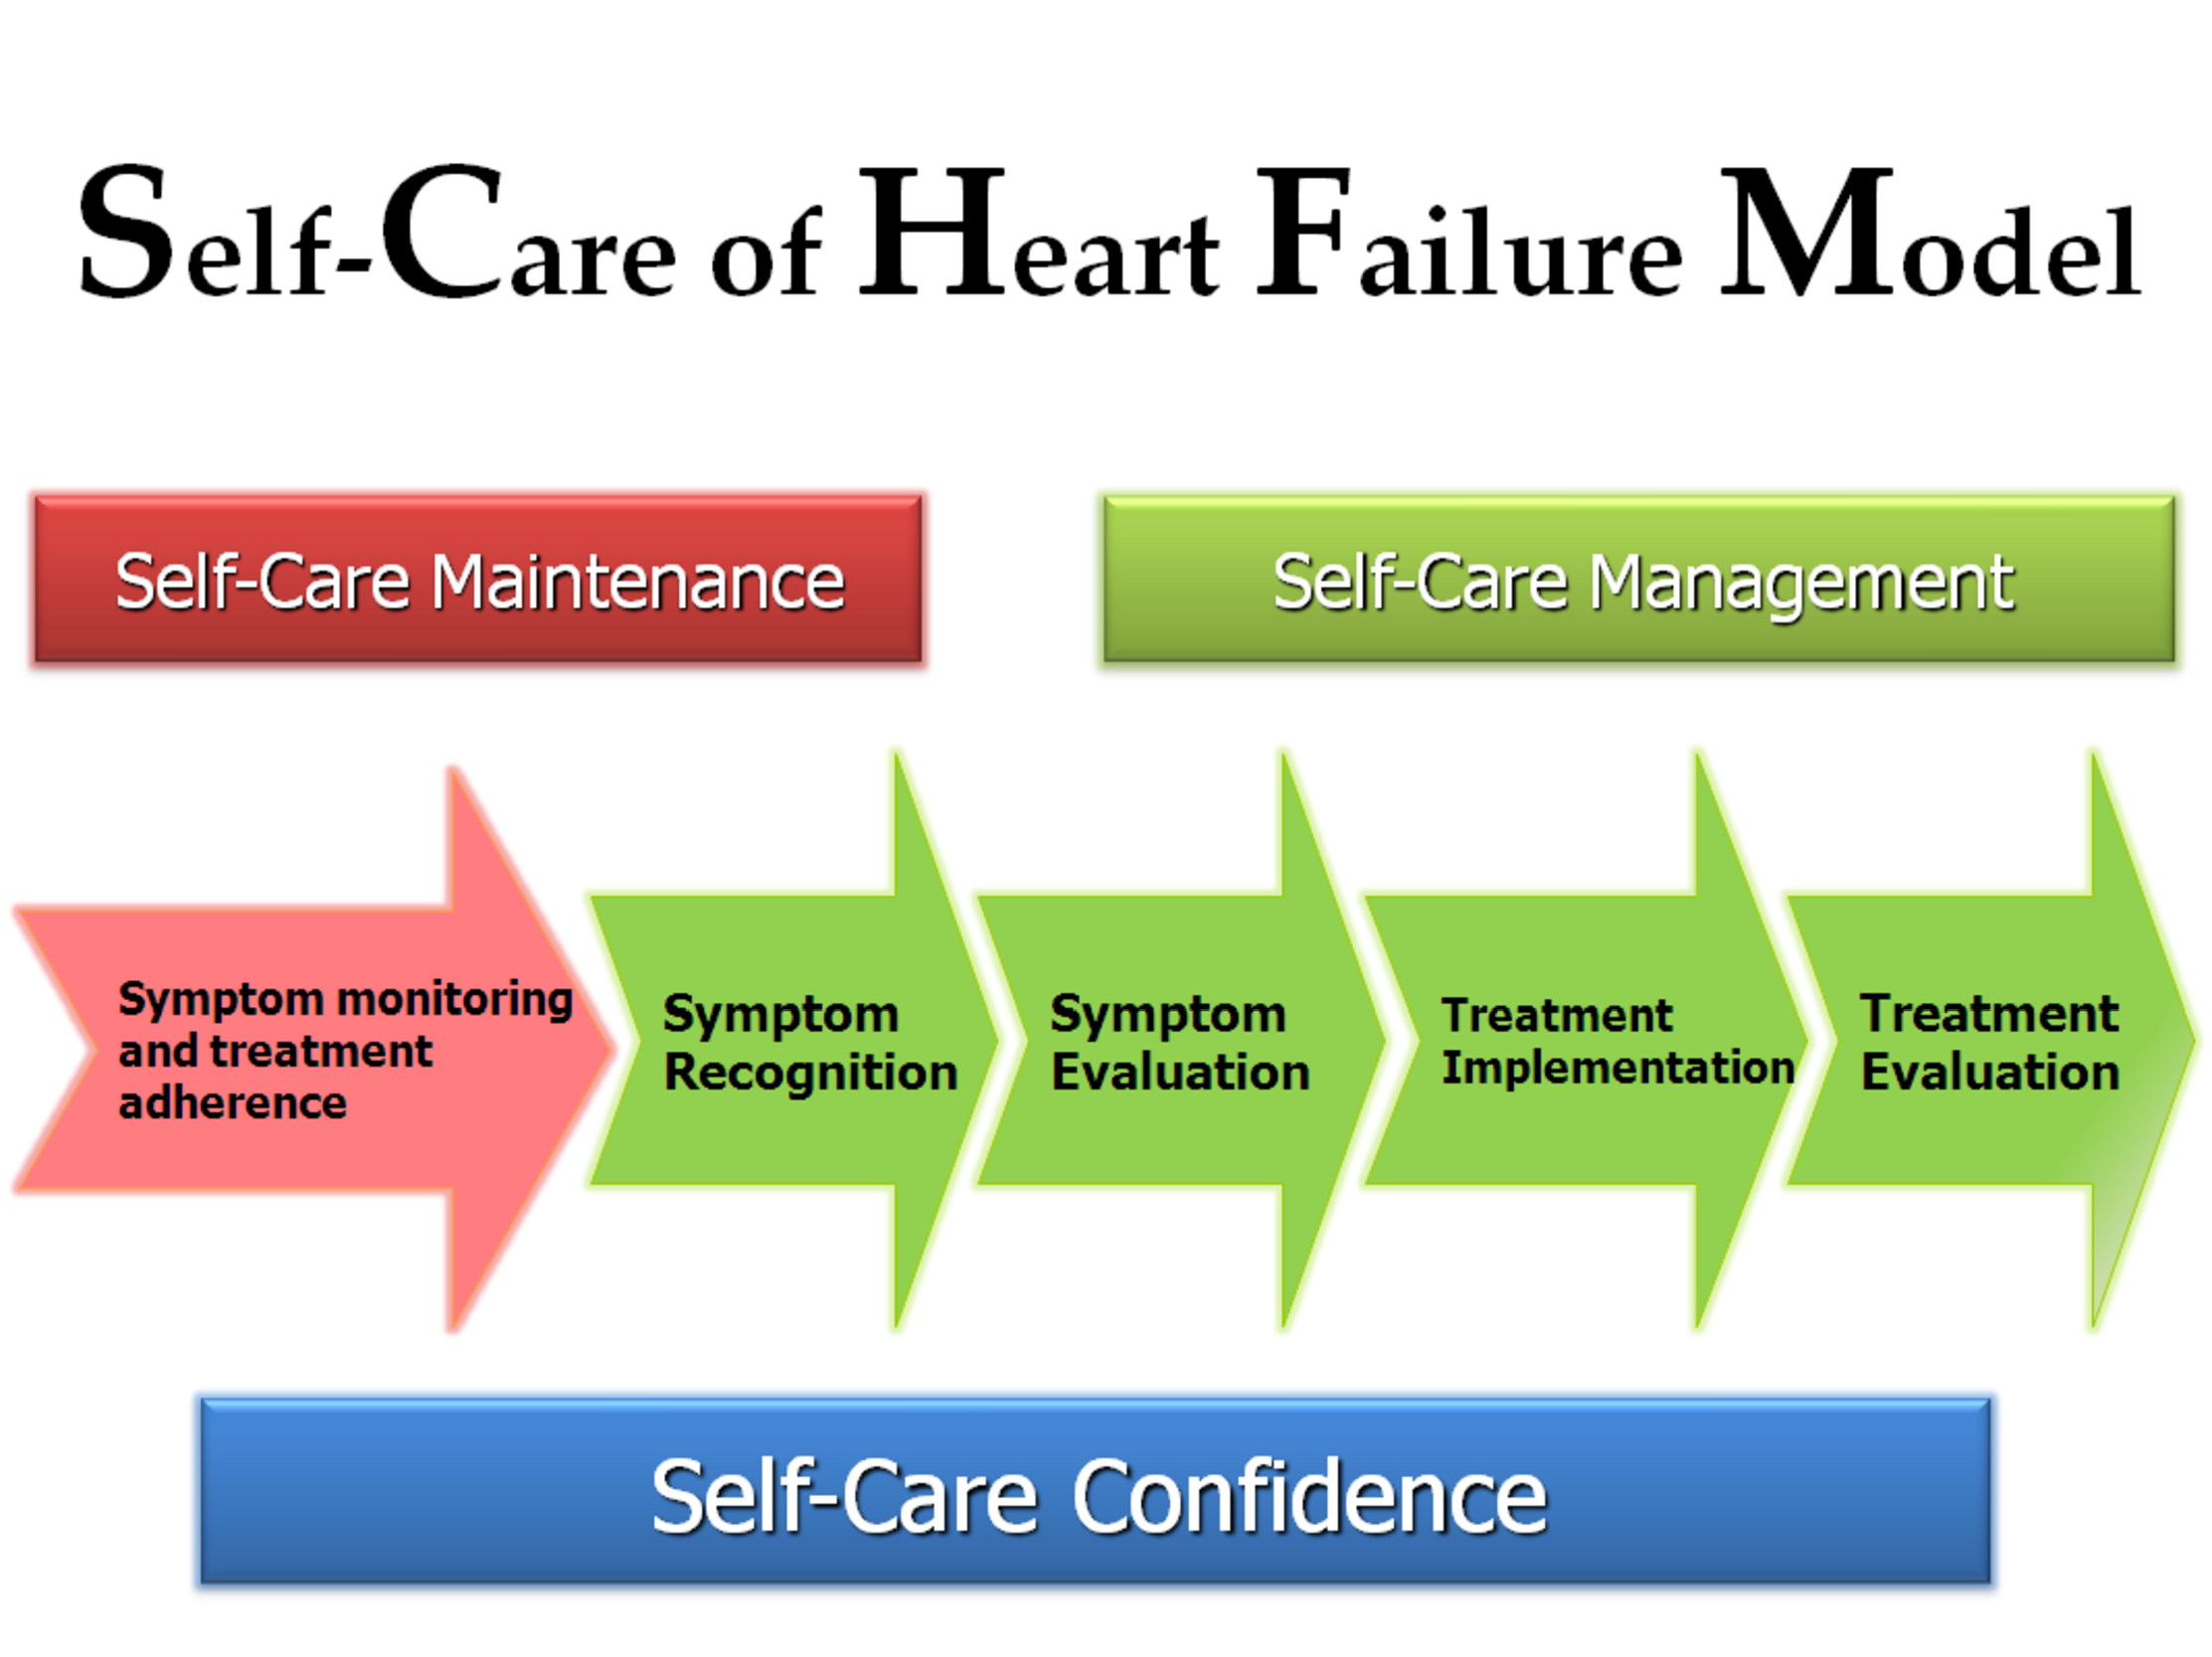
\includegraphics[scale=1,width=0.9\textwidth]{Images/SelfCare_cropped.pdf} 
		\caption{Theory of HF Self-Care }
	\end{center}
\end{figure}

With alerts to notify clinicians of an imminent event (an emergency) or a downward trend in need of correction, the WHIPPED system allows medical professionals to more effectively monitor a greater number of patients without degrading care. WHIPPED further provides a continuous link between patient and clinician which improves on the current visitation model, prescribed by Medicare, indicating that a home visit is needed after discharge and typically extends to ninety days post discharge \cite{Dansky2008}.

The dissertation will address the design, implementation, and testing of the WHIPPED Systems' three parts: the WHIP sensor, the cellphone application, and the Back-end Knowledge Engine. The dissertation will also discuss the exploratory study, conducted by Dr. Sethares and its role in validating the WHIPPED System.

\section{Importance of topic}
\label{sec:importanceOfTopic}

\begin{figure}
	\begin{center}
		\label{fig:DaysofCare}
		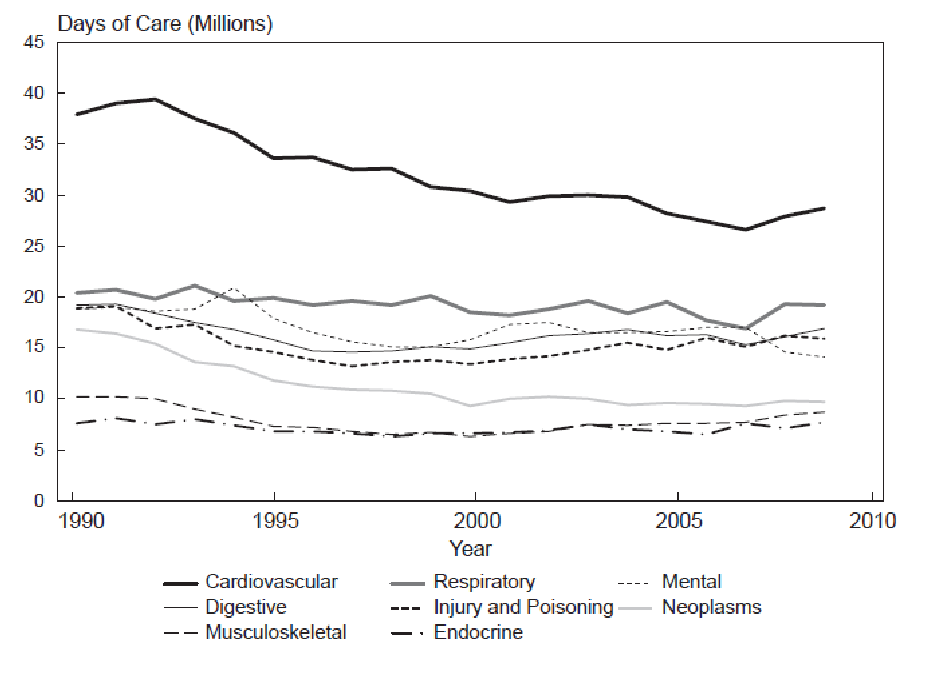
\includegraphics[scale=1,width=0.9\textwidth]{Images/DaysOfCare.png} 
		\caption{Number of days of inpatient hospital care by major diagnosis U.S., 1990-2009 }
	\end{center}
\end{figure}

Mussilino, working for the National Institutes of Health, compiled statistical data for the number of days of hospital care, required for different illnesses shown in  \cref{fig:DaysofCare} \cite{Mussolino2012}. Cardiovascular disease is clearly a major cost concern. Therefore, reducing re-hospitalization rates can substantially reduce the cost of cardiac care.


\begin{figure}
	\begin{center}
		\label{fig:SurvivalRates}
		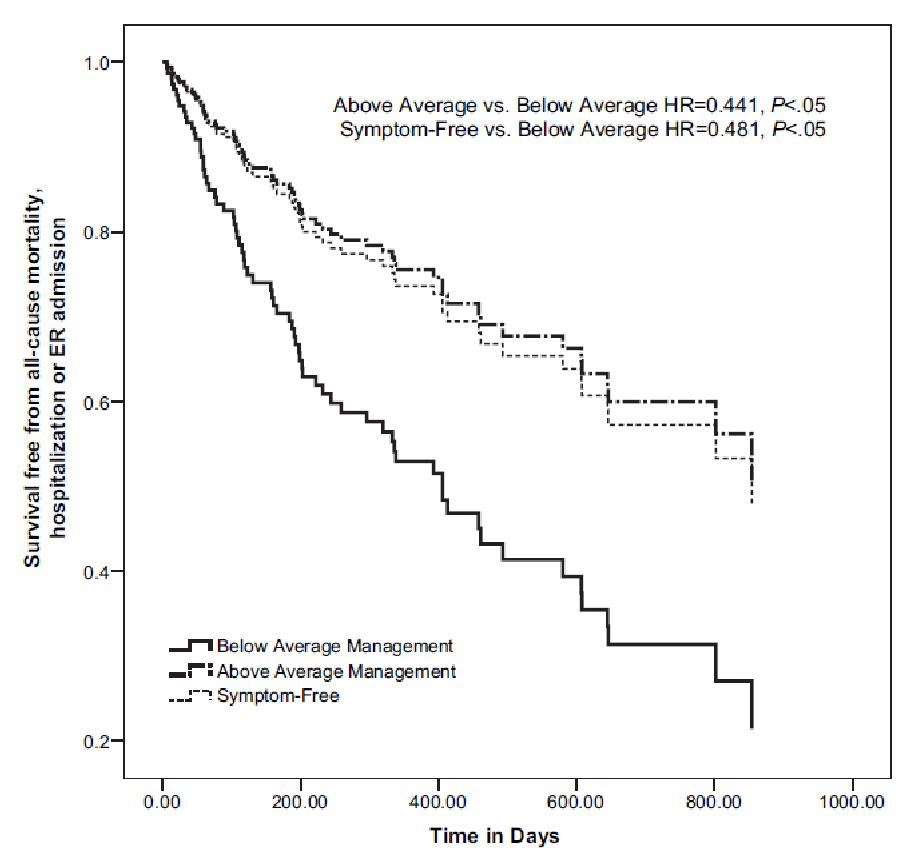
\includegraphics[scale=1,width=0.9\textwidth]{Images/SurvivalRate.jpg} 
		\caption{Survival Rates Of Patients Who Engage In Self Care Versus Those That Do Not.}
	\end{center}
\end{figure}

\begin{verse}
NOTE: timmy makes a case, the boys make a case..... is Lee et al. plural?
\end{verse}

Lee et al. make a compelling case concerning patients who engage in self-care management \cref{fig:SurvivalRates}. \cite{Lee2011} The benefits of actively engaging patients in their own self-care can clearly be seen in their research.   Patients engaged in self-care management cut in half their risk of death, hospitalization, and need for emergency treatment compared to patient not involved in their own care. Furthermore, self-care managed patients with high-risk profiles were also shown to be nearly equivalent to patient who were symptom free \cite{Lee2011}.

Sethares and Elliott conduct a study providing tailored educational messages to patients to induce healthy self-care behaviors \cite{Sethares2004249}. Sethares and Elliot assess patient's QOL in their study using the Minnesota Living with Heart Failure questionnaire (MLHF). These tailored educational messages, from now on called interventions, were designed to encourage patients to engage in self-care such as taking medication on time, following a low sodium diet, etc. The statistical analysis showed patients were more likely to engage in self-care behaviors given these tailored message interventions. The study also did not show a significant decrease in re-hospitalizations. 
\begin{quote}
NOTE: yes this is a true fact.


"A Kruskall-Wallis test was run to answer research
question 1. HF readmission rate was not signifi-
cantly related to group assignment in this study ( P
ϭ .22). As seen in Table IV, 12 subjects in the
control group were rehospitalized 1 or more times,
whereas 6 subjects in the treatment group were
rehospitalized 1 or more times."
\end{quote}

However, one of the limitations of Sethares and Elliott's study, the inability to monitor actual self-care behaviors, suggests an avenue for improvement, or augmentation of the tailored message interventions. Several other proven instruments for measuring perceived patient status exist including the Heart Failure Somatic Awareness (HFSA) \cite{Jurgens2006} test and the Duke Activity Status Index (DASI) \cite{Hlatky1989}. Using a combination of the MLHF, HFSA, and DASI instruments, self-care management can be augmented by allowing treatment evaluation \cref{fig:SelfCare}.   

According to Mussolino, Cardiovascular diseases were the leading cause of hospitalization for at least the past two decades. Moreover the cost of cardiovascular disease in 2008, as outlined in \cref{fig:CVDCost}, was \$297.7 billion \cite{Mussolino2012}. If patients are involved in their own self-care, and made aware of their state of wellness, so they can act on it and affect change, the financial strain on the health-care system can be greatly reduced. Some research to provide automated educational material to patients based on clinical practice guidelines (CPGs) showed promise \cite{Jones2005}. Further research, directed at producing protocols, based on best evidence practices, more accessible and editable by medical professionals emphasizes their need and value \cite{Shah2001}.

\begin{figure}
	\begin{center}
		\label{fig:CVDCost}
		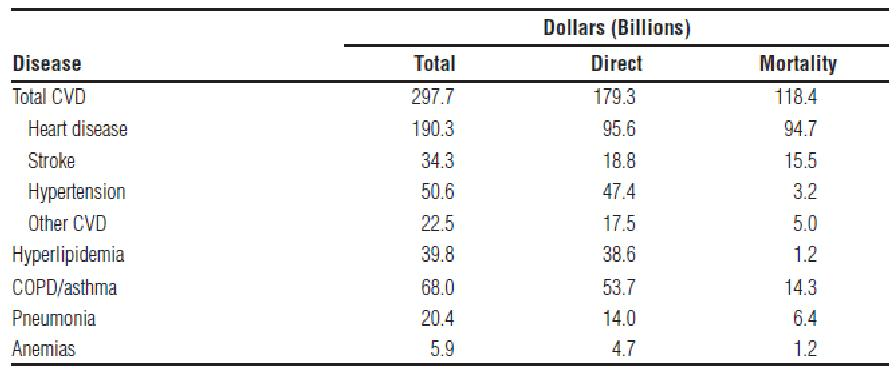
\includegraphics[scale=1,width=0.9\textwidth]{Images/CostOfCVD.jpg} 
		\caption{Economic Cost of Cardiovascular, Lung, and Blood diseases U.S., 2008 }
	\end{center}
\end{figure}

\section{Problem Statement}
\label{sec:problemStatement}
The evidence presented, indicates a need for the WHIPPED system. WHIPPED collects both the psychosocial data from instruments like the HFSA, DASI, and MLHF and biometric data from the wireless sensor suite.  WHIPPED correlates the collected data to provide more timely feedback to a patient in the first days, weeks and months of their discharge from the hospital after a HF related event as needed. WHIPPED must have as little physical impact on a user as possible. WHIPPED utilizes non-invasive synthetic sensor technologies to derive common cardiac metrics using a minimal number of physical measurements. 

Currently, disparate research exists to collect cardiac metrics with an acceptable level of accuracy given only one or two transducers. The goal of the dissertation is the design, implementation, and testing/validation of the complete end-to-end WHIPPED system. Key features of the system are:

\begin{itemize}
\item The use of synthetic sensor measurements to detect cardiac metrics, specifically ECG, \spo2, blood pressure, respiration, and heart rate.
\item A hardware, firmware, and software implantation of a cardiac sensor suite.
\item The development of a wellness measure, to classify and indicate patient's cardiac heath and overall wellness. \cite{Chaiyasucheeva2012}
\item The ability to offer interventions to engage a patient in self-care.
\item Remote monitoring capabilities for clinicians, offering direct interaction with patients.
\end{itemize}

In addition, the dissertation develops techniques for fusing the collected information, consulting with a CPG or specialized cardiac ontology and providing cardiac-wellness feedback to engage a patient in their self-care regimen. Using feedback and motivated self-interventions patients can follow up on their conditions with more rigor than currently possible given current institutional and personnel limitations, possibly at a greatly reduced cost. Additionally, a system is proposed whereby medical professionals can monitor patient's wellness, to offer additional interventions as needed.

\section{Hypothesis}
\label{sec:Hypothesis} 

NOTE: this is the hypothesis made, before the research, so does it use future tense?

In the dissertation research, we are designing, developing, and testing an end-to-end system, along with proposing an exploratory study using a mix of technologies, proven evidence based practices, interventions to aid patients in learning about and becoming involved in home self-care. During the dissertation's research, we will determine if technology can assist patients to understand their own illness, and act to improve their QOL and decrease the chance of re-hospitalization. 

Subsequently, when designing and experimenting with the WHIPPED system we propose to answer several questions. First, will patients use the technology? Second, will the technology aid patients in understanding their disease?  Third, can patients learn to act in improving their overall wellness? When considering adoption of the technology we propose looking at the smartphone by itself, the smartphone and sensor suite, the sensors themselves and a control group. If patients fully adopt the system, both the smartphone for its psychosocial elements and the sensors for the physiologic data, most robust analysis can be performed. Full technology adoption may allow us to answer, possibly, another question; is there a correlation between perceived wellness, as reported using the psychosocial data, and actual wellness, derived through sensor measurements? If the patient only uses the smartphone, no physiologic data can be gathered and only the perceived status of the patient can be discerned. Similarly, if the patient does not complete any of the psychosocial questionnaires only the biometric readings will be available. The dissertation hypothesizes we can improve patient QOL, reduce the need for re-hospitalization, and therefore lower costs by implementing the proposed system, primarily by educating the patient, using evidence based best practice philosophies.


\section{Research Approach}

NOTE: this is the research approach that was outlined before the research was performed, so does it use future tense?

In order to actualize the WHIPPED system the design is divided into three parts: the sensor suite, the smartphone application, and the BKE. Each piece will be designed and the interfaces between each part specified. Before designing can take place however, the responsibilities of the system must be divided and the requirements of the system must be applied to each part of the system.

The sensor suite is envisioned as a wearable patch, requiring no advanced medical knowledge to apply. Furthermore, since it is the main physical part of the system, and the goal of the system is to be low cost, the sensor suite must be as low cost as possible. The device will implement sensors to collect real-time ECG and \spo2 measurements to satisfy these requirements. The system will be responsible for deriving all other physiological measurements. The sensor suite should be small, battery powered, and capable of wireless communication with the smartphone. 

The smartphone will perform three main functions. First, it will receive and retransmit the biometric data to BKE, capable of mining the received data. Second, the smartphone will periodically assess the patient using psychosocial instruments, such as the DASI and HFSA, further augmenting the data received from the sensors. The third, and final, task of the smartphone is to receive data from the BKE. The BKE can deliver a calculated wellness measure, auto generated tailored interventions, medical reminders (e.g. take medication), or messages from the clinician. We seek to validate good behavior on the part of the patient and discourage unhealthy behavior by providing the wellness measure to the patient. 

Auto-generated interventions will not provide suggestions requiring a clinician, such as a prescription, but will instead be changes to the CHF patient's lifestyle, such as diet or exercise, to increase the wellbeing and the longevity of the patient while decreasing the risk of re-hospitalization. 

Patients will be able to view their wellness, ECG, \spo2, respiration, and heart rate history as temporal graphs. Temporal graphs will aid patient's learning about how their activity (e.g. adherence to interventions, taking medications) affects their overall wellbeing.

The BKE will make use of a minimal cardiac ontology with co-morbidity information to assess a patient's status. The wellness metric will be based on the collected biometric readings as well as the psychosocial instruments correlated with the medical ontology to calculate the patient's overall wellness. We will also track the patient's wellness over time, and, if a decreasing trend is detected in the patient's wellness score, provide possible interventions to the user to reverse the downward trend. Finally, in severe cases we can provide an alert to a medical professional indicating immediate care is needed.

Having defined the requirements and operation of the system, focus can now switch to realization. The natural first choice is to construct a sensor platform to collect ECG and PPG readings. The "\nameref{sec:ResearchDoneToDate}" section shows significant progress in data collection has been achieved. While building the sensor suite, work also began on several smartphone applications. Early applications were responsible for displaying collected data in real time in order to validate the sensor designs. Work can begin on the design of the BKE, after sensor suite validation. The BKE is partitioned into four design tasks. 
\begin{itemize}
\item First a minimal EHR was designed and implemented. Identification of co-morbidities and demographic data storage are the primary goals of the initial EHR.
\item The second task will be to expand the EHR to support real-time biometric data and periodic psychosocial data. 
\item The third task is to design and implement a minimal cardiac ontology.
\item Lastly, the algorithms for wellness calculation and interventions can be implemented using data provide for the first three parts.
\end{itemize}
These four tasks will not be completed atomically. Part of building and validating a database is providing test data. The other parts of the system, the smartphone and WHIP, can be integrated with each BKE task. A smartphone app allowing “registration” can be written, after designing a minimal EHR , with the intention of integration into the final smartphone application. Once the EHR is expanded to support the sensor and psychosocial data, integrating the three parts of the system together can begin. Firmware for the sensor can be written, designed to transfer the data to the smartphone.  The smartphone will have a service to relay the sensor data to the BKE. The smartphone will also be able to administer psychosocial instruments. 
A secondary smartphone application can be written, geared towards a clinicians use, to monitor the data coming from the sensor suite. Once the data transfer to the BKE is tested and verified the task of wellness calculation and intervention analysis can begin. Validation of the back-end computations is accomplished using simulated patient data input into the database. Patient simulations will seek to test the wellness calculations validity. The smartphone app will be augmented to receive data from the BKE and deliver the wellness calculation to the patient simulation. The BKE will also be presented with simulated patients who have decreasing wellness scores and will be tested to see what types of interventions are provided. The emergency feature of the system can be implemented and tested without the BKE; designed to call an urgent care center if a cardiac event, such as a heart attack, is detected. If the sensor suite detects such an event, it should send an alert to the smartphone. The phone can then place a call and automatically deliver information such as location, type of event detected, and patient information to the operator. The phone can then connect the operator to the patient if they are conscious, to allow further information to be communicated. During testing of the emergency response feature another number can be substituted for 911. Then a simulated event can be input into the system to test if the event is detected and the phone call placed. Once the functionality of these devices has been verified, an exploratory research study is proposed to validate the system with real world participants.

\section{Limitations and key assumptions}
\label{sec:LimitationsAndKeyAssumptions}
The WHIPPED system could be expanded to many domains. However, we bound the research in several areas. When we move to real world patients, we will seek between ten and twenty participants for an experimental study, not a clinical trial. A study allows us to select patients who will most benefit from the system, specifically patients over sixty-five who have had one or more cardiac events. We are further limiting ourselves in the area of design to consider non-invasive methods of data collection. While there have been long-term implantable devices developed [54], these are not suitable for the dissertation's purposes. Creating a system having the smallest possible impact on the day-to-day activities of the patient is significant goal of the research. Therefore, any device which connects to a patient, must be in a small form factor. If the device is to be removable, it must not require any special knowledge to re-affix the device.  Furthermore, the device should be designed with long-term use in mind. Since the device must be portable, battery power is needed. Battery power further implies the device must be low power.

\section{Contributions to knowledge}
\label{sec:ContributionsToKnowledge}
Due to the interdisciplinary nature of this dissertation, contributions can be split into two areas: the contributions to the medical domain and the contributions to the engineering domain. The medical domain can benefit by using the WHIPPED system to test the hypothesis that engaging patients in their own self-care can lead to a better QOL and reduce hospitalization. During the exploratory study, tests will be performed based on patients who use the traditional care method (the control), patients using only the psychosocial instruments, and patients who have the sensors and psychosocial instruments. We can also access if patients will effectively use the system to facilitate their self-care.
For the engineering domain, we will develop new and novel techniques for data fusion and knowledge acquisition supporting numerous future applications (e.g. future soldier systems, athlete training). We will design implement and validate an end-to-end system that integrates synthetic sensors, wireless communication, and the calculation of a wellness measure, using an EHR and BKE into an all-inclusive system. We will provide a medical solution to engage patients in their own self-care cheaply with little impact on the user. The WHIPPED solution can reduce health-care costs and increase QOL. 

\section{Research Done To Date}
\label{sec:ResearchDoneToDate}
In preparation for the main research component of my dissertation, we have already performed some preliminary work in the fields of bio-sensing. The first step was to get up to speed on the research group's status. During the 2009-2010 school years, a senior design group was tasked with building an analog front end to capture an ECG signal. Also, during the 2009-2010 school years, master's candidate Osama Aljaroudi designed an analog front-end excitation and conditioning circuit for a \spo2/PPG circuit. A device with both circuits was designed and fabricated on a four-layer PCB board and shown in \cref{fig:PCB_alpha}. Unfortunately, because of the inexperience with the tools the board suffered from many problems. These were eventually rectified with “green wire fixes”. A great deal was learned from the initial foray into fabrication.

\begin{figure}
	\begin{center}
		\label{fig:PCB_alpha}
		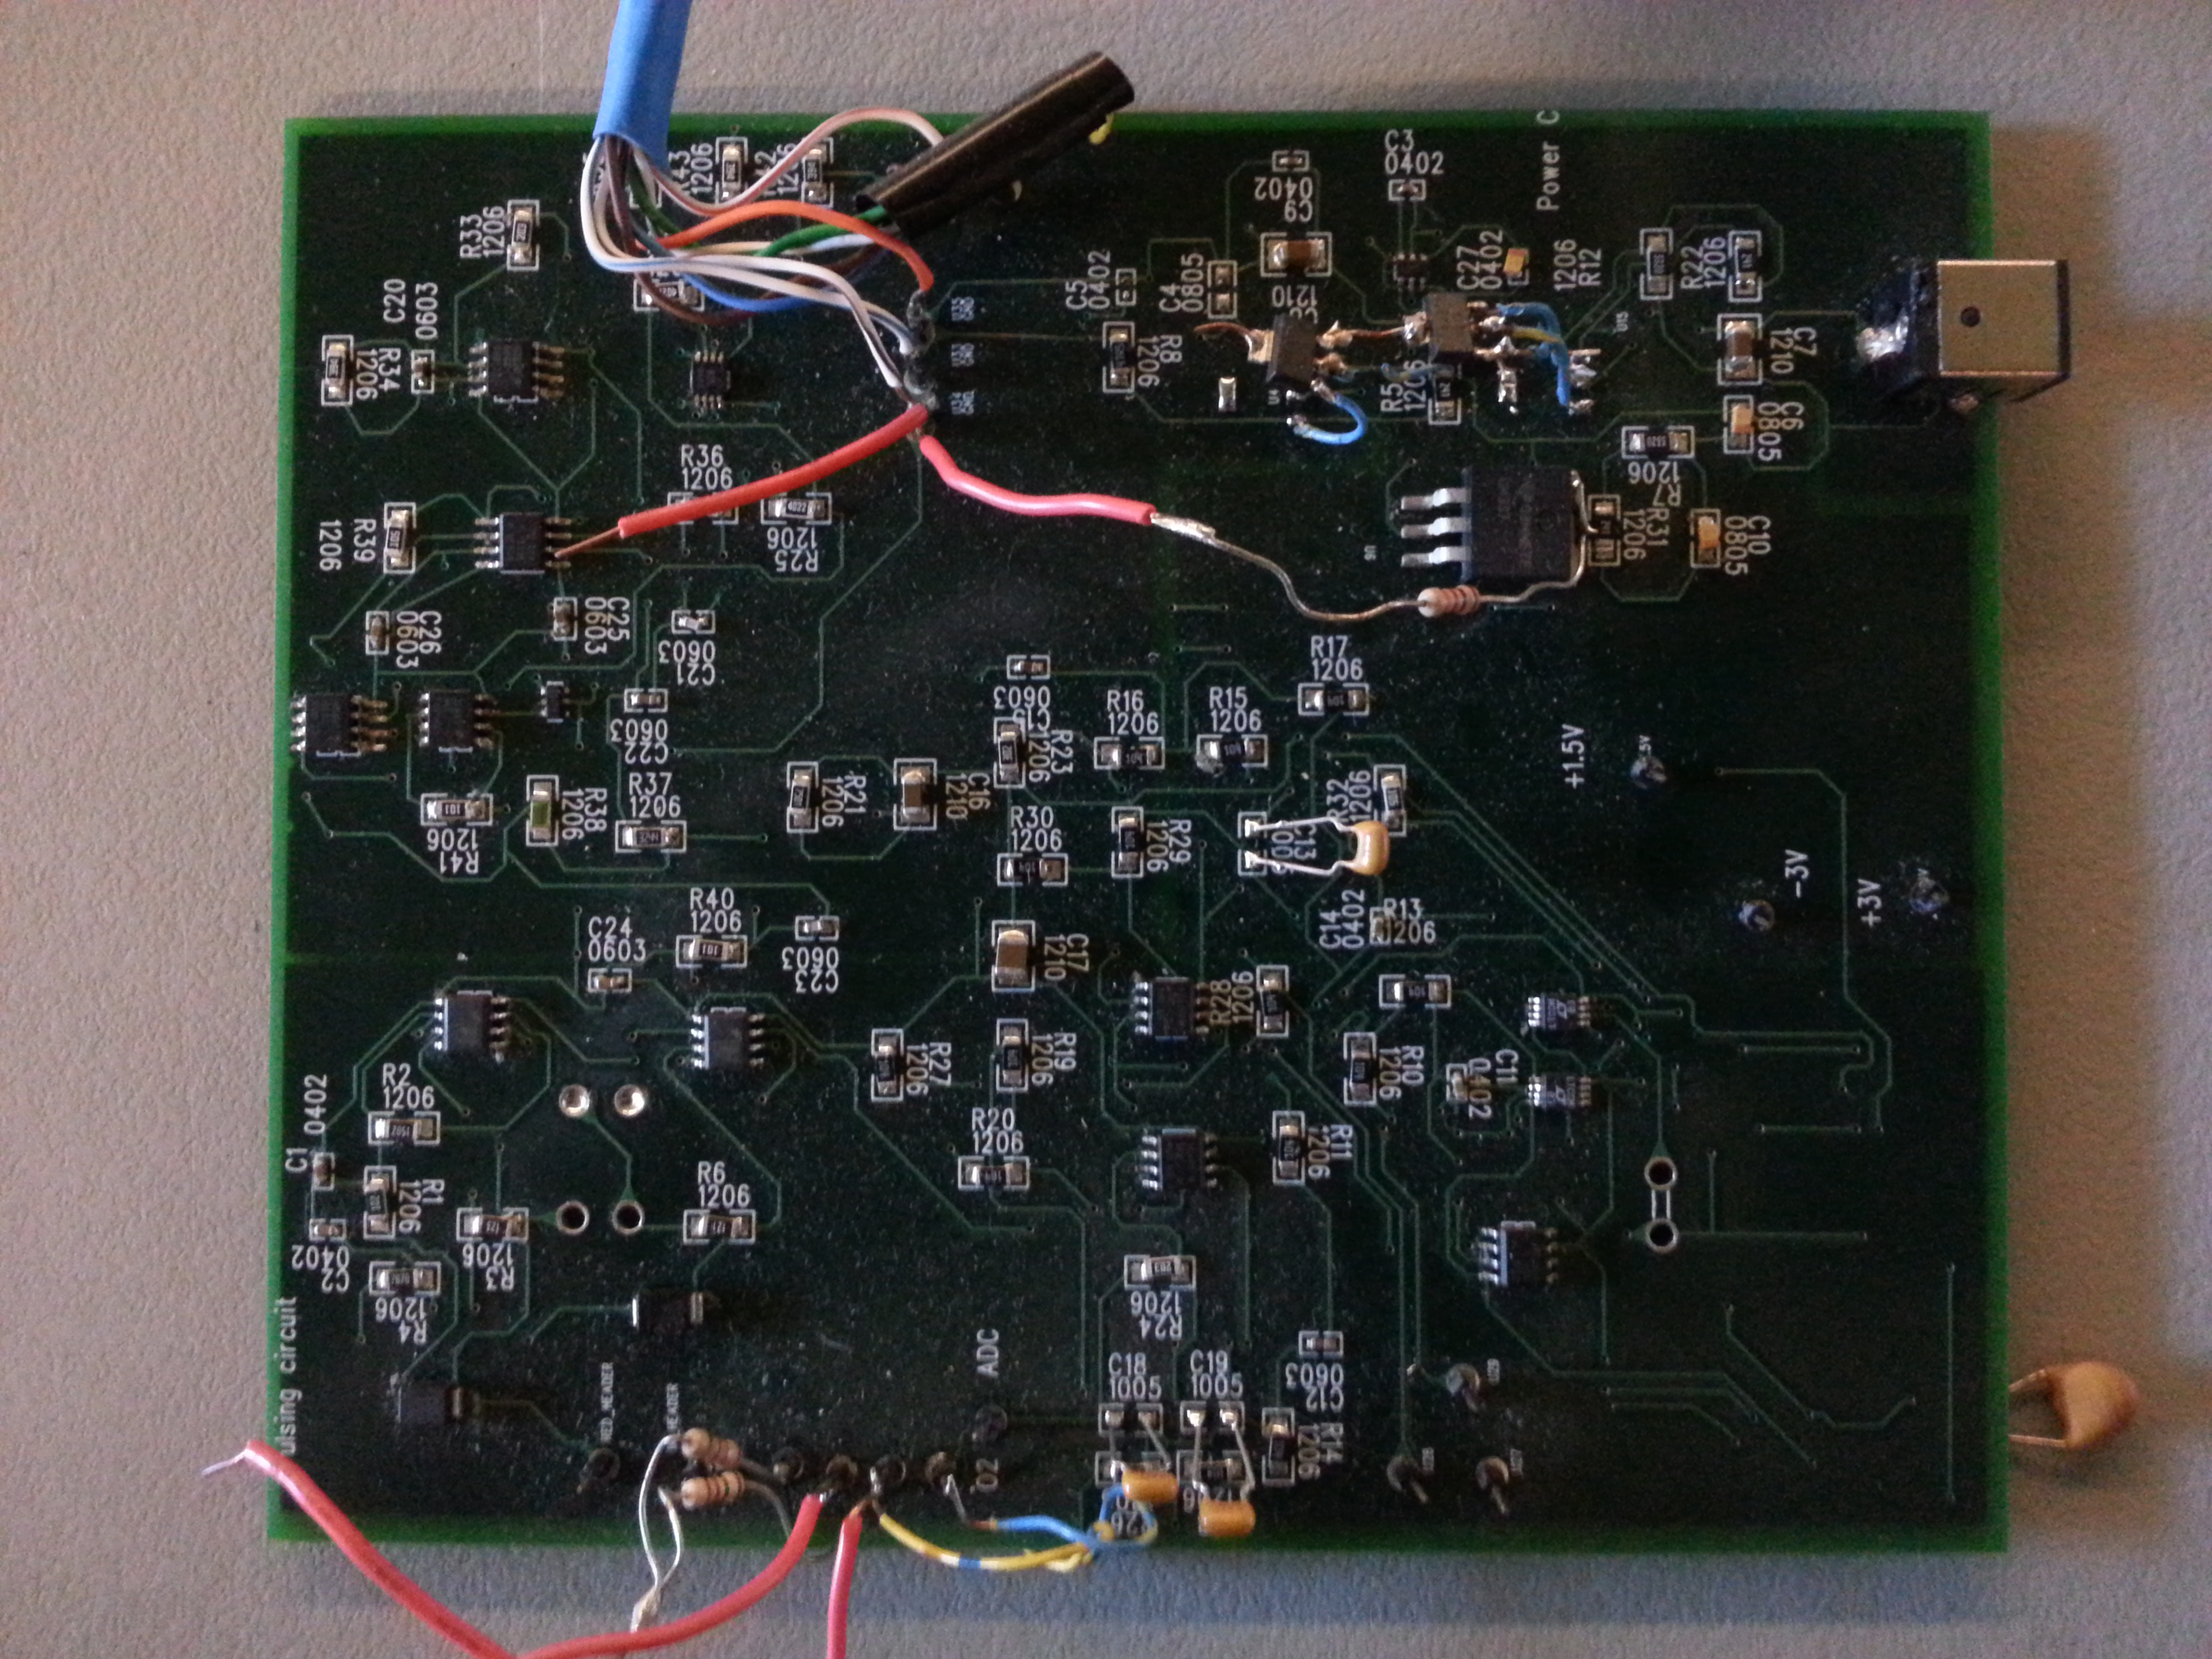
\includegraphics[scale=1,width=0.9\textwidth]{Images/PCB_Alpha.jpg} 
		\caption{Analog front-end alpha board.}
	\end{center}
\end{figure}

The next revision of the hardware was personally undertaken by me in the spring of 2011. Referred to as Revision Alpha, the design miniaturized the footprint of the analog front end. The design utilized an adaptation of the senior design group's ECG circuit and the master candidate's \spo2 circuit. Alpha's design utilized surface mount integrated circuits (ICs) and through-hole passive components. The prototype sensors were fabricated as a two-layer board shown in \cref{fig:PCB_analog_beta}. Some calculated resistances needed to be fabricated by soldering some components to each other “dead-bug” style due to lack of available stock. The lesson learned: check what parts are available before finalizing a design.

\begin{figure}
	\begin{center}
		\label{fig:PCB_analog_beta}
		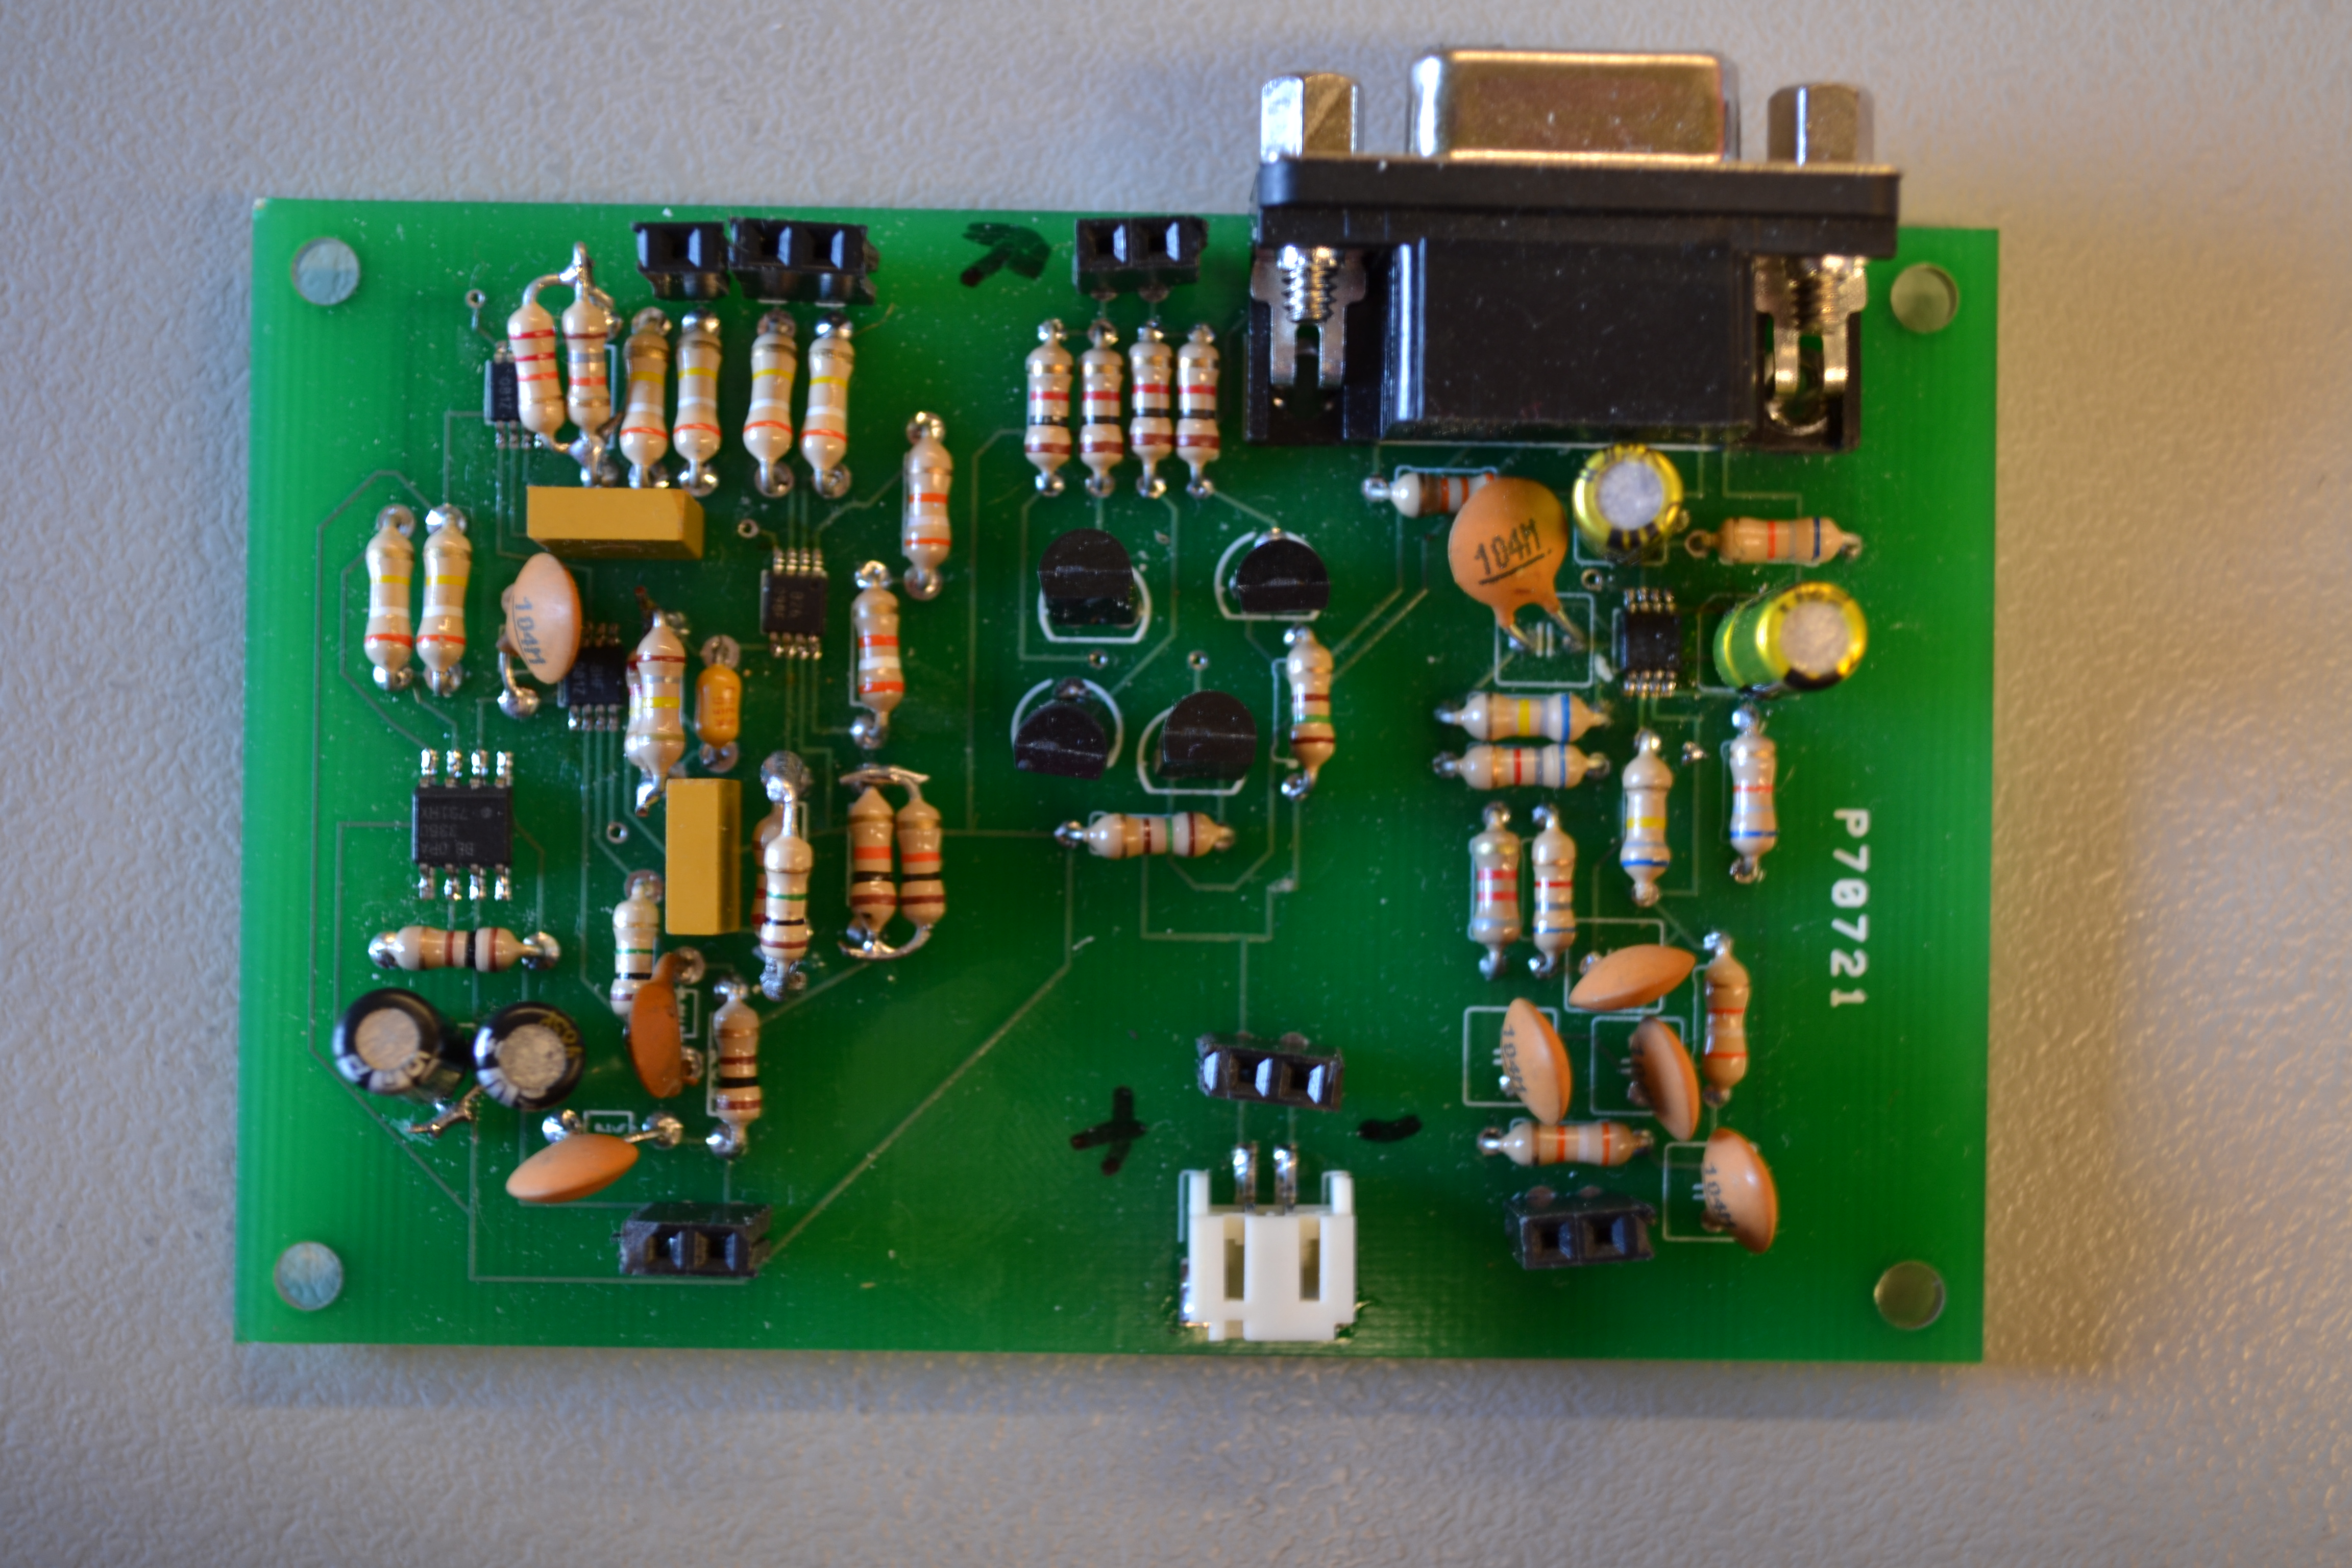
\includegraphics[scale=1,width=0.9\textwidth]{Images/PCB_AnalogBeta.JPG} 
		\caption{Beta Analog board}
	\end{center}
\end{figure}

To interact with the analog front-end board a controller PCB was manufactured in-house to host an ADuC7020 development socket. This board was designed in the same fashion, using the same tools as the analog front-end board but was manufactured by hand using an acid etching process and drilled on my CNC router (designed to improve the turnaround time and cost of prototypes). Front and back views are shown in \cref{fig:PCB_digital_beta}. The controller board served to validate the results of the initial analog designs. Using results from early prototyping work began on the first revision of an integrated solution. This board integrated as many components as possible into the sensor design.

\begin{figure}
	\begin{center}
		\label{fig:PCB_digital_beta}
		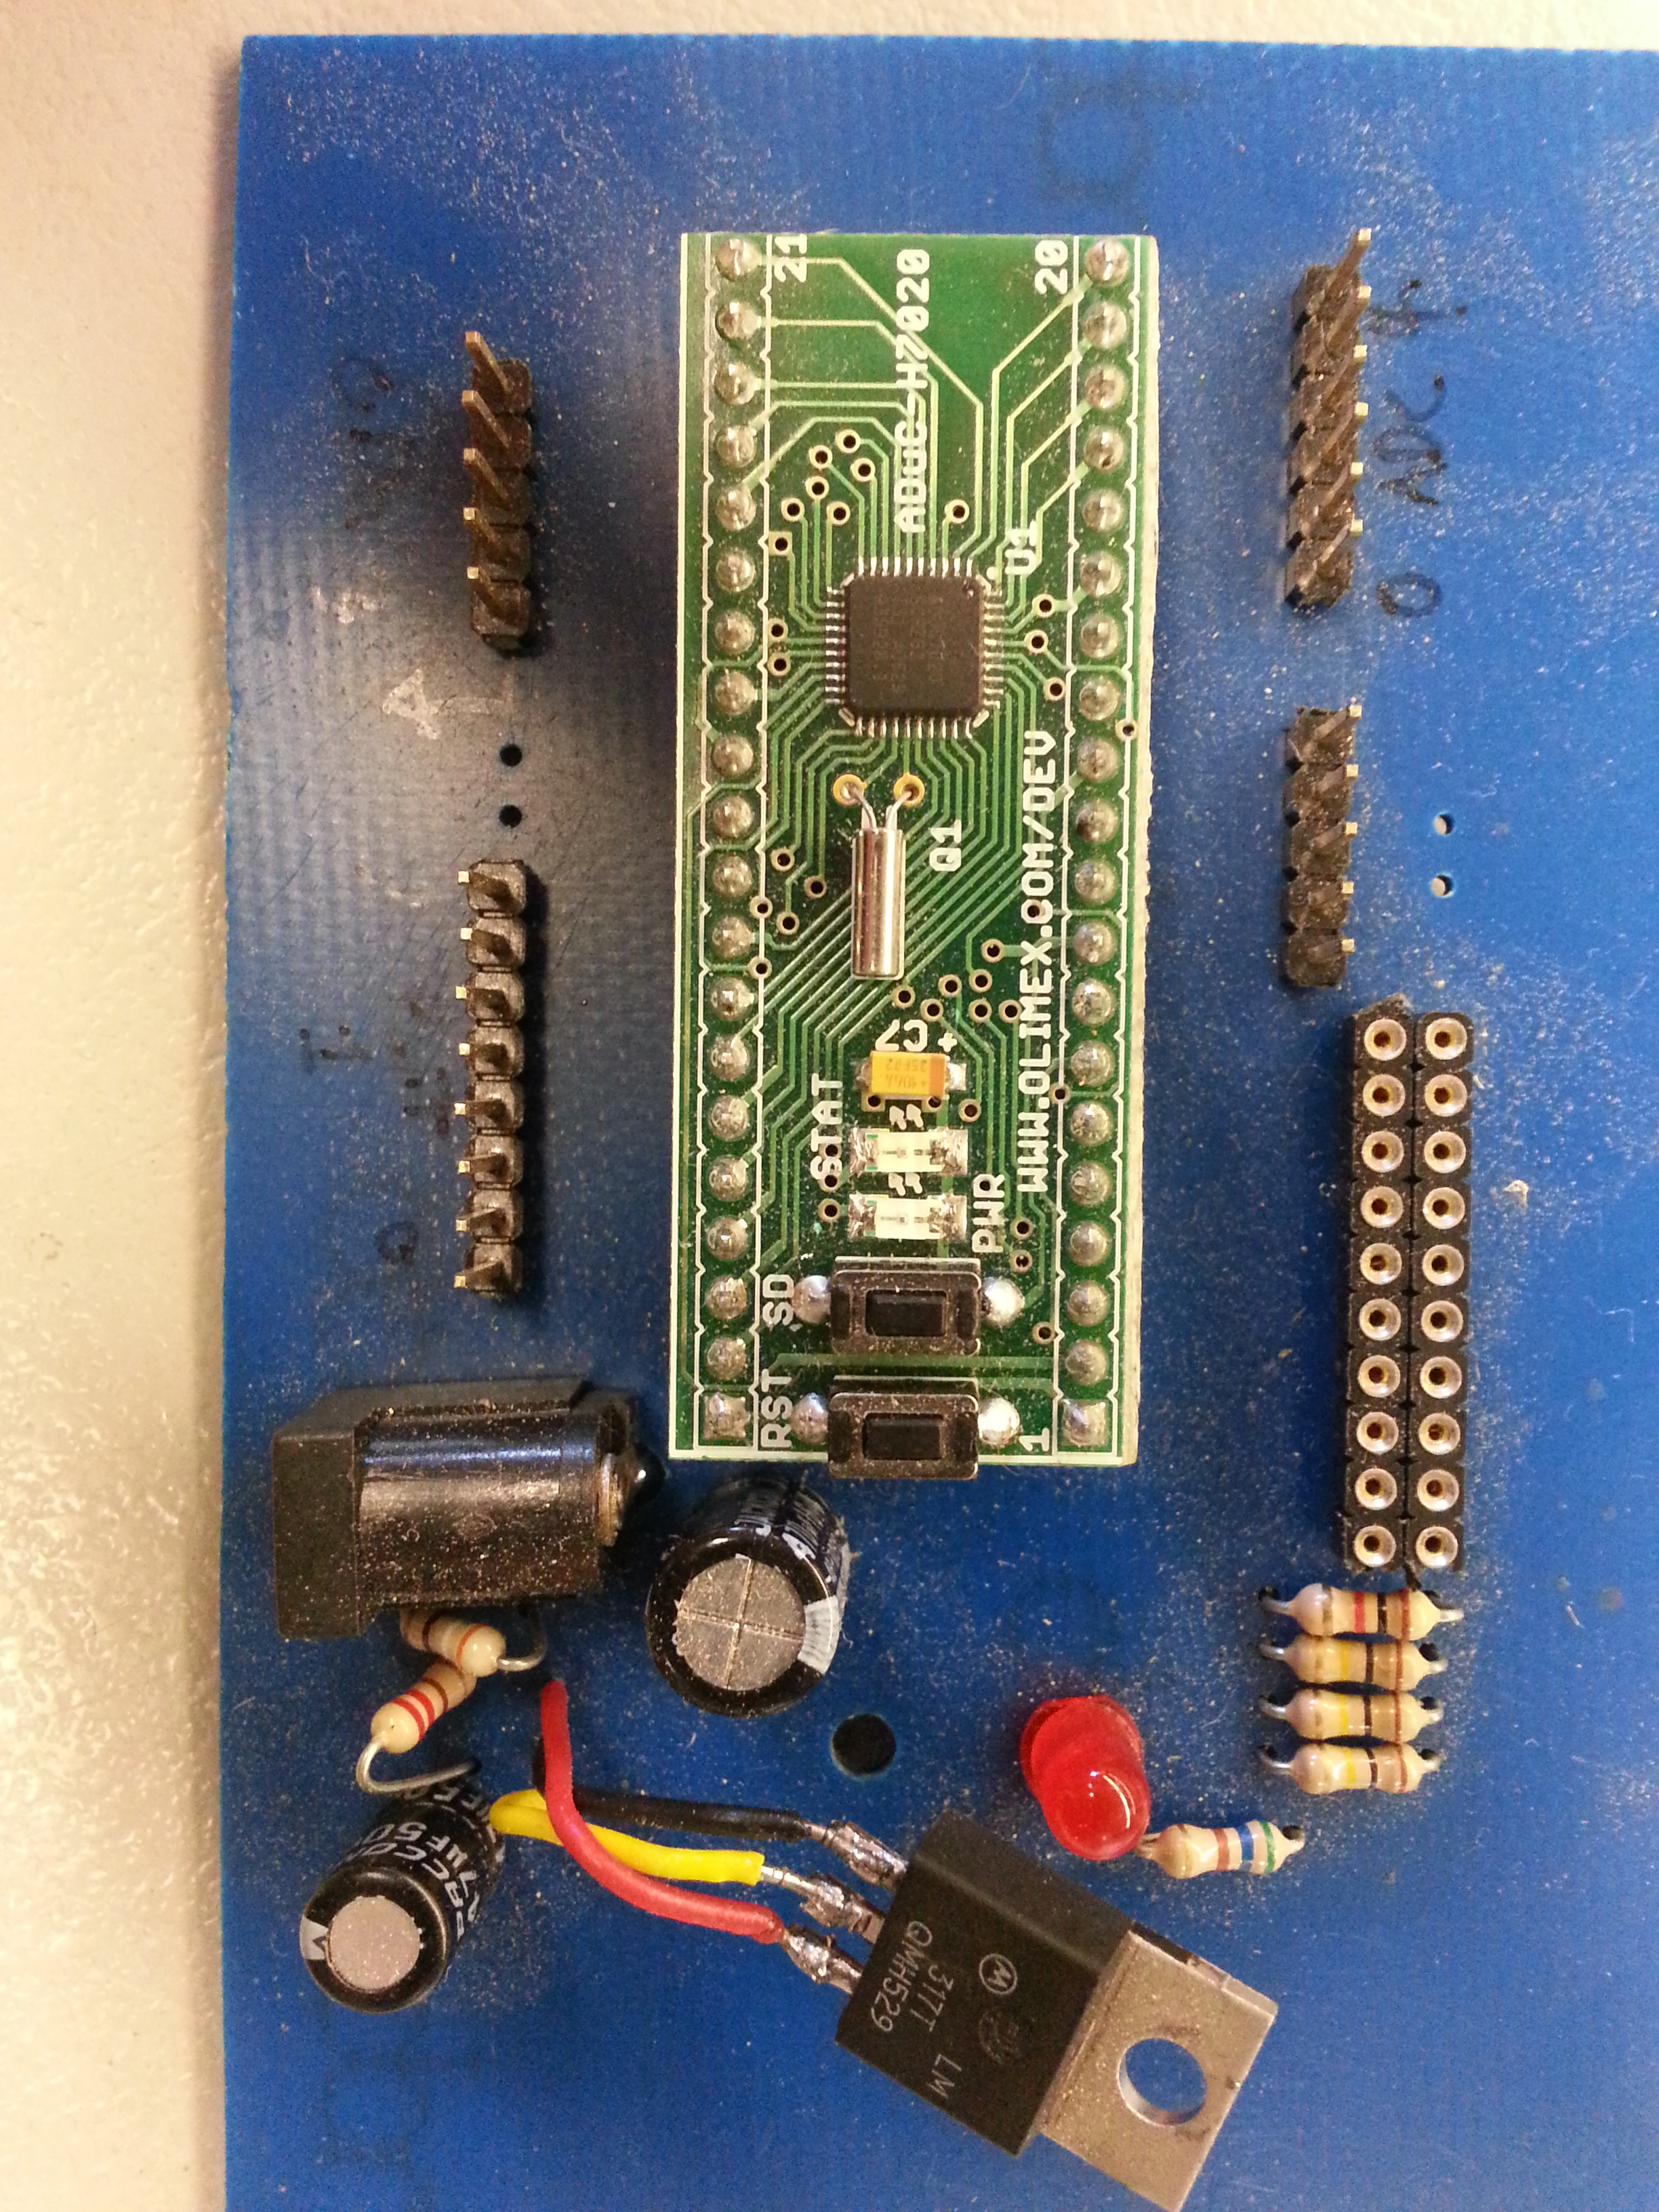
\includegraphics[scale=1,width=.45\textwidth]{Images/PCB_DigBetaA.jpg}
		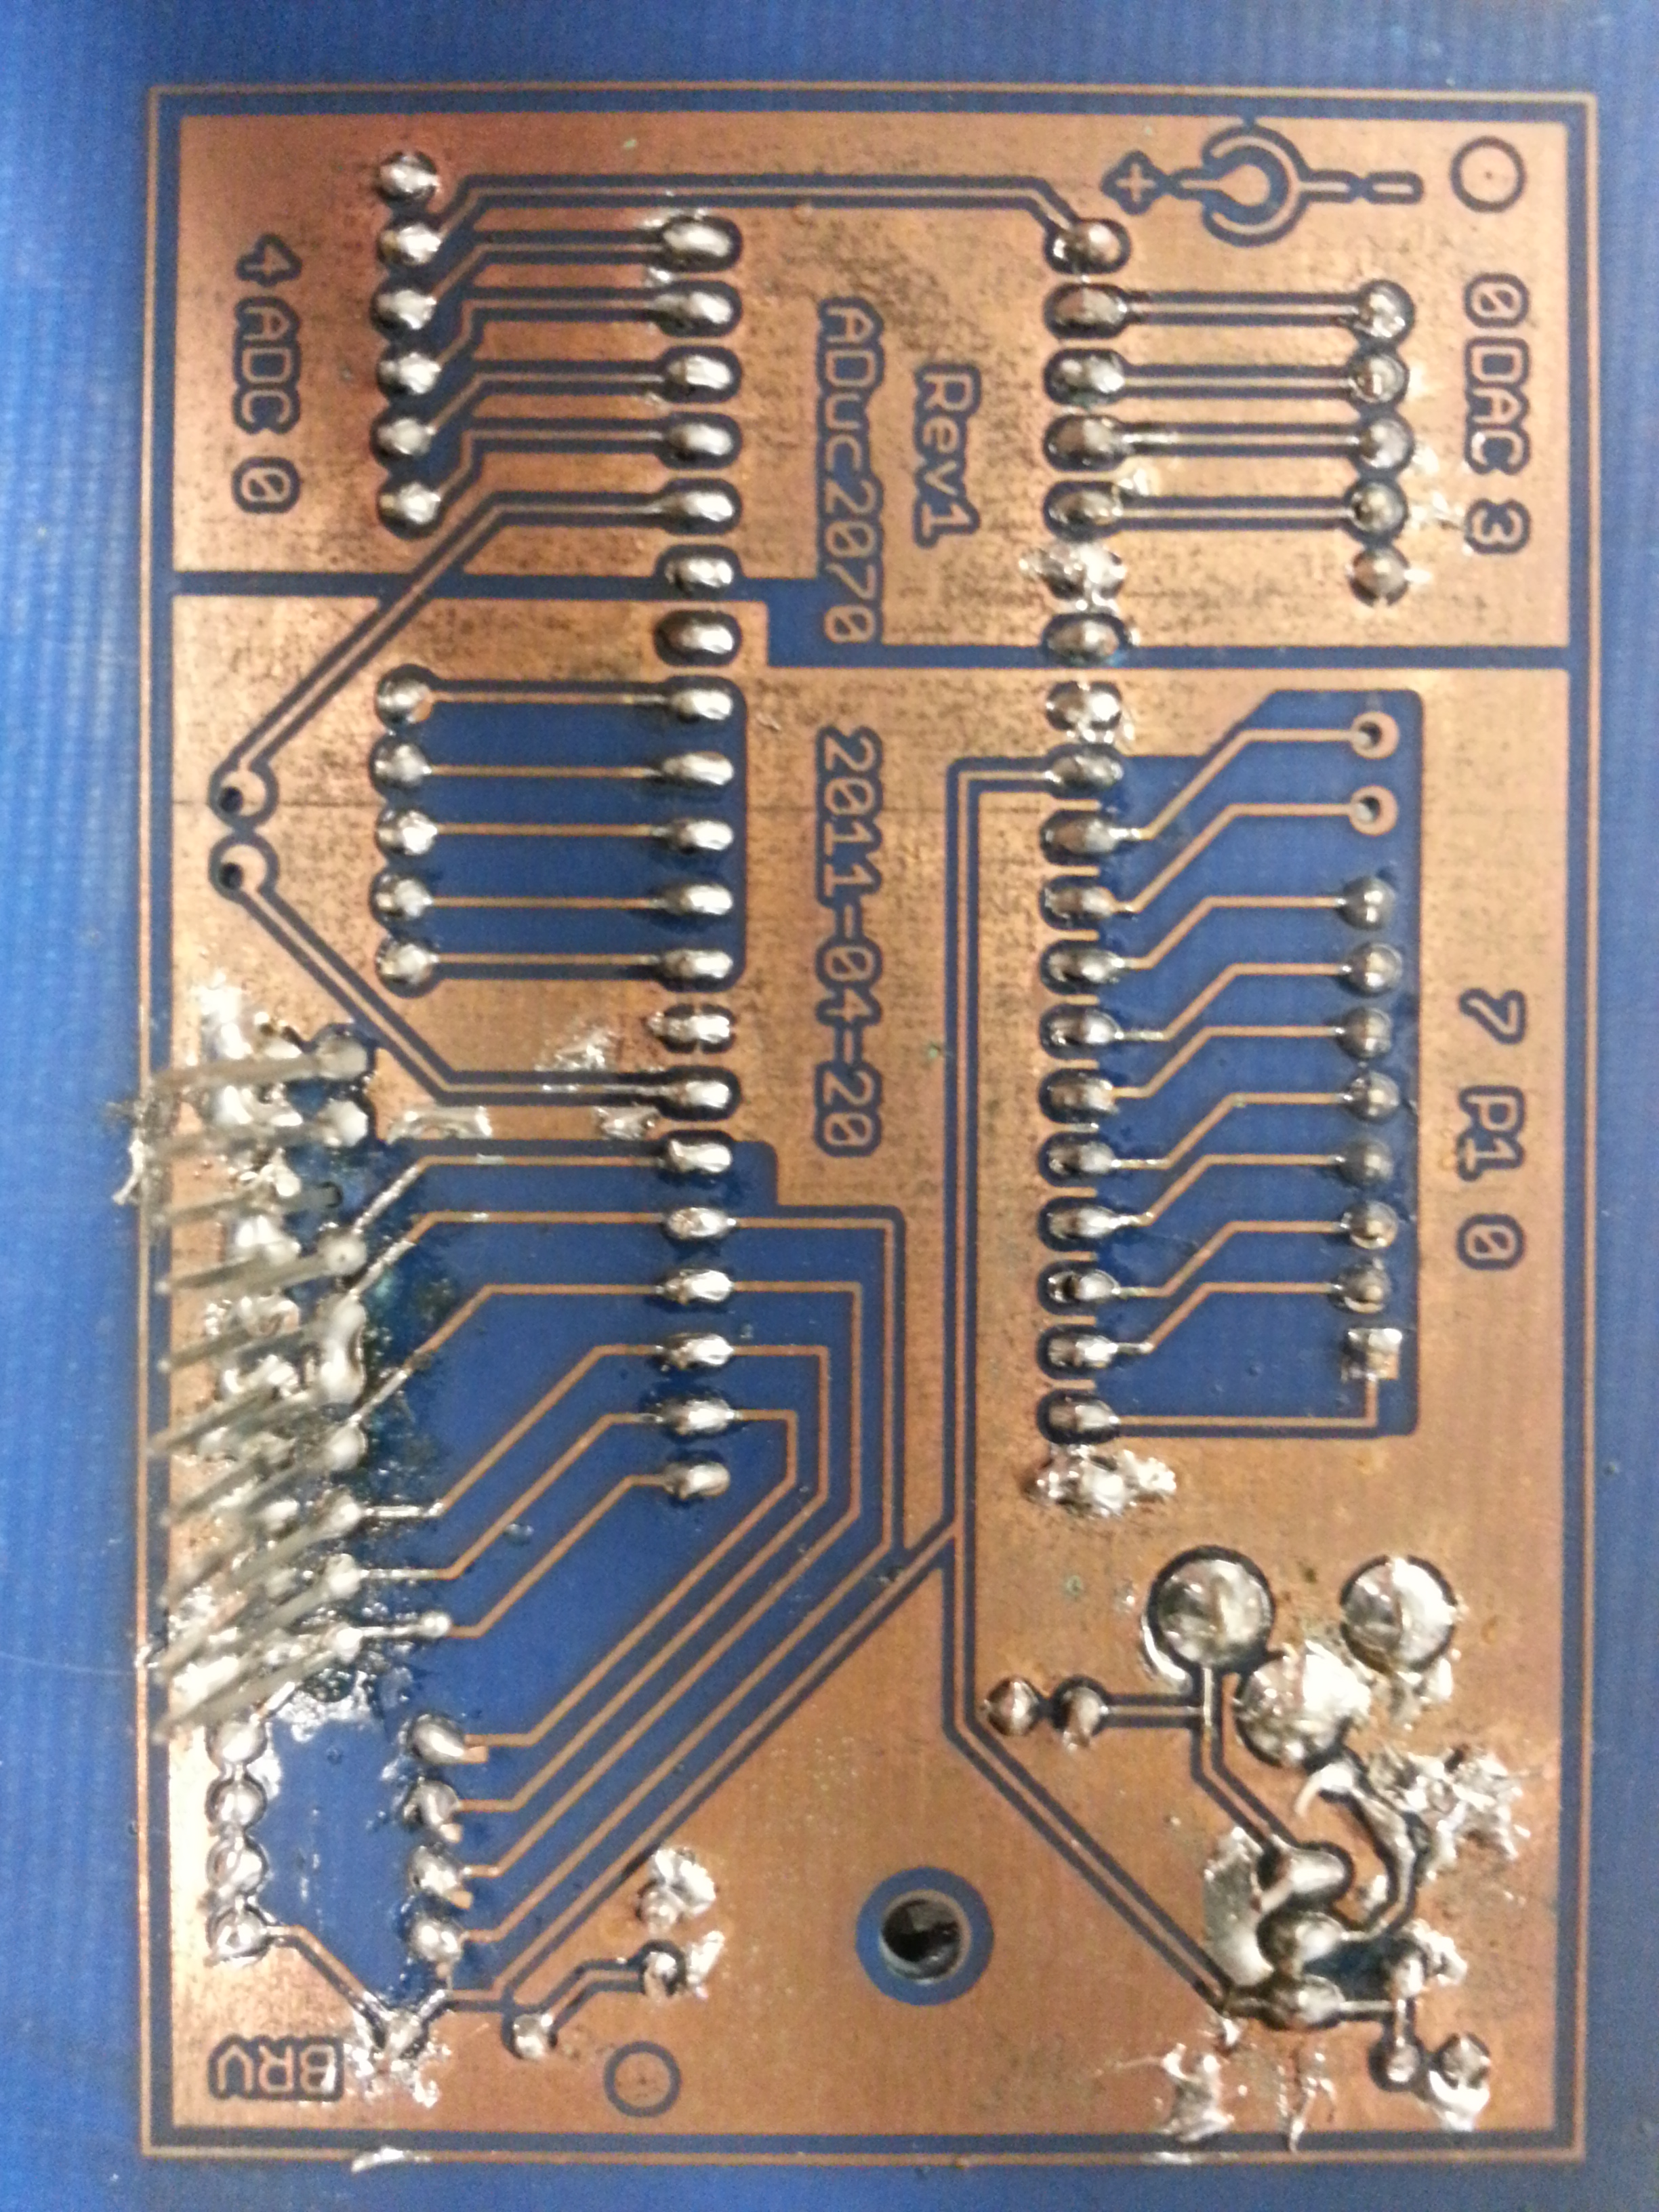
\includegraphics[scale=1,width=.45\textwidth]{Images/PCB_DigBetaB.jpg}  
		\caption{Beta Control Board}
	\end{center}
\end{figure}

To clarify the different parts of the design the hardware device was referred to as the Mobile Cardiac Heart Monitor (MCHM). This first revision, shown in \cref{fig:PCB_Rev1}, was designed as a test platform. It included many peripherals including an accelerometer, Bluetooth-communication, USB-communication, SD card storage, and an integrated  Lithium Polymer (LiPo) battery charger in addition to the previously designed analog front end. The board also transitioned to surface mount parts. This board was assembled and tested. Once basic functionality of all components was verified, We began to work towards miniaturization of the device. This effort would attempt to streamline the design; reducing points of failure, cost, complexity, and size.  Revision 2 (Rev2) was never manufactured due to a supplier mix-up. The processor had been advertised with an incorrect footprint. It was determined to be cheaper to have new boards manufactured using the altered footprint than to wait for new processor. The revised board was called revision 3 (Rev3), shown in \cref{fig:PCB_Rev3}, functionally identical to revision 2 but with a different microprocessor footprint. Rev3 added the feature of a connector that could easily be affixed to ECG leads without proprietary devices. Rev3 also could function as a full nine degrees of freedom sensor (9DOF). This was used for another researcher's master thesis [16]. Finally, a new \spo2 sensor was being developed by a master student, the original design was removed, and a header was added for connection to any design the student could create.

\begin{figure}
	\begin{center}
		\label{fig:PCB_Rev1}
		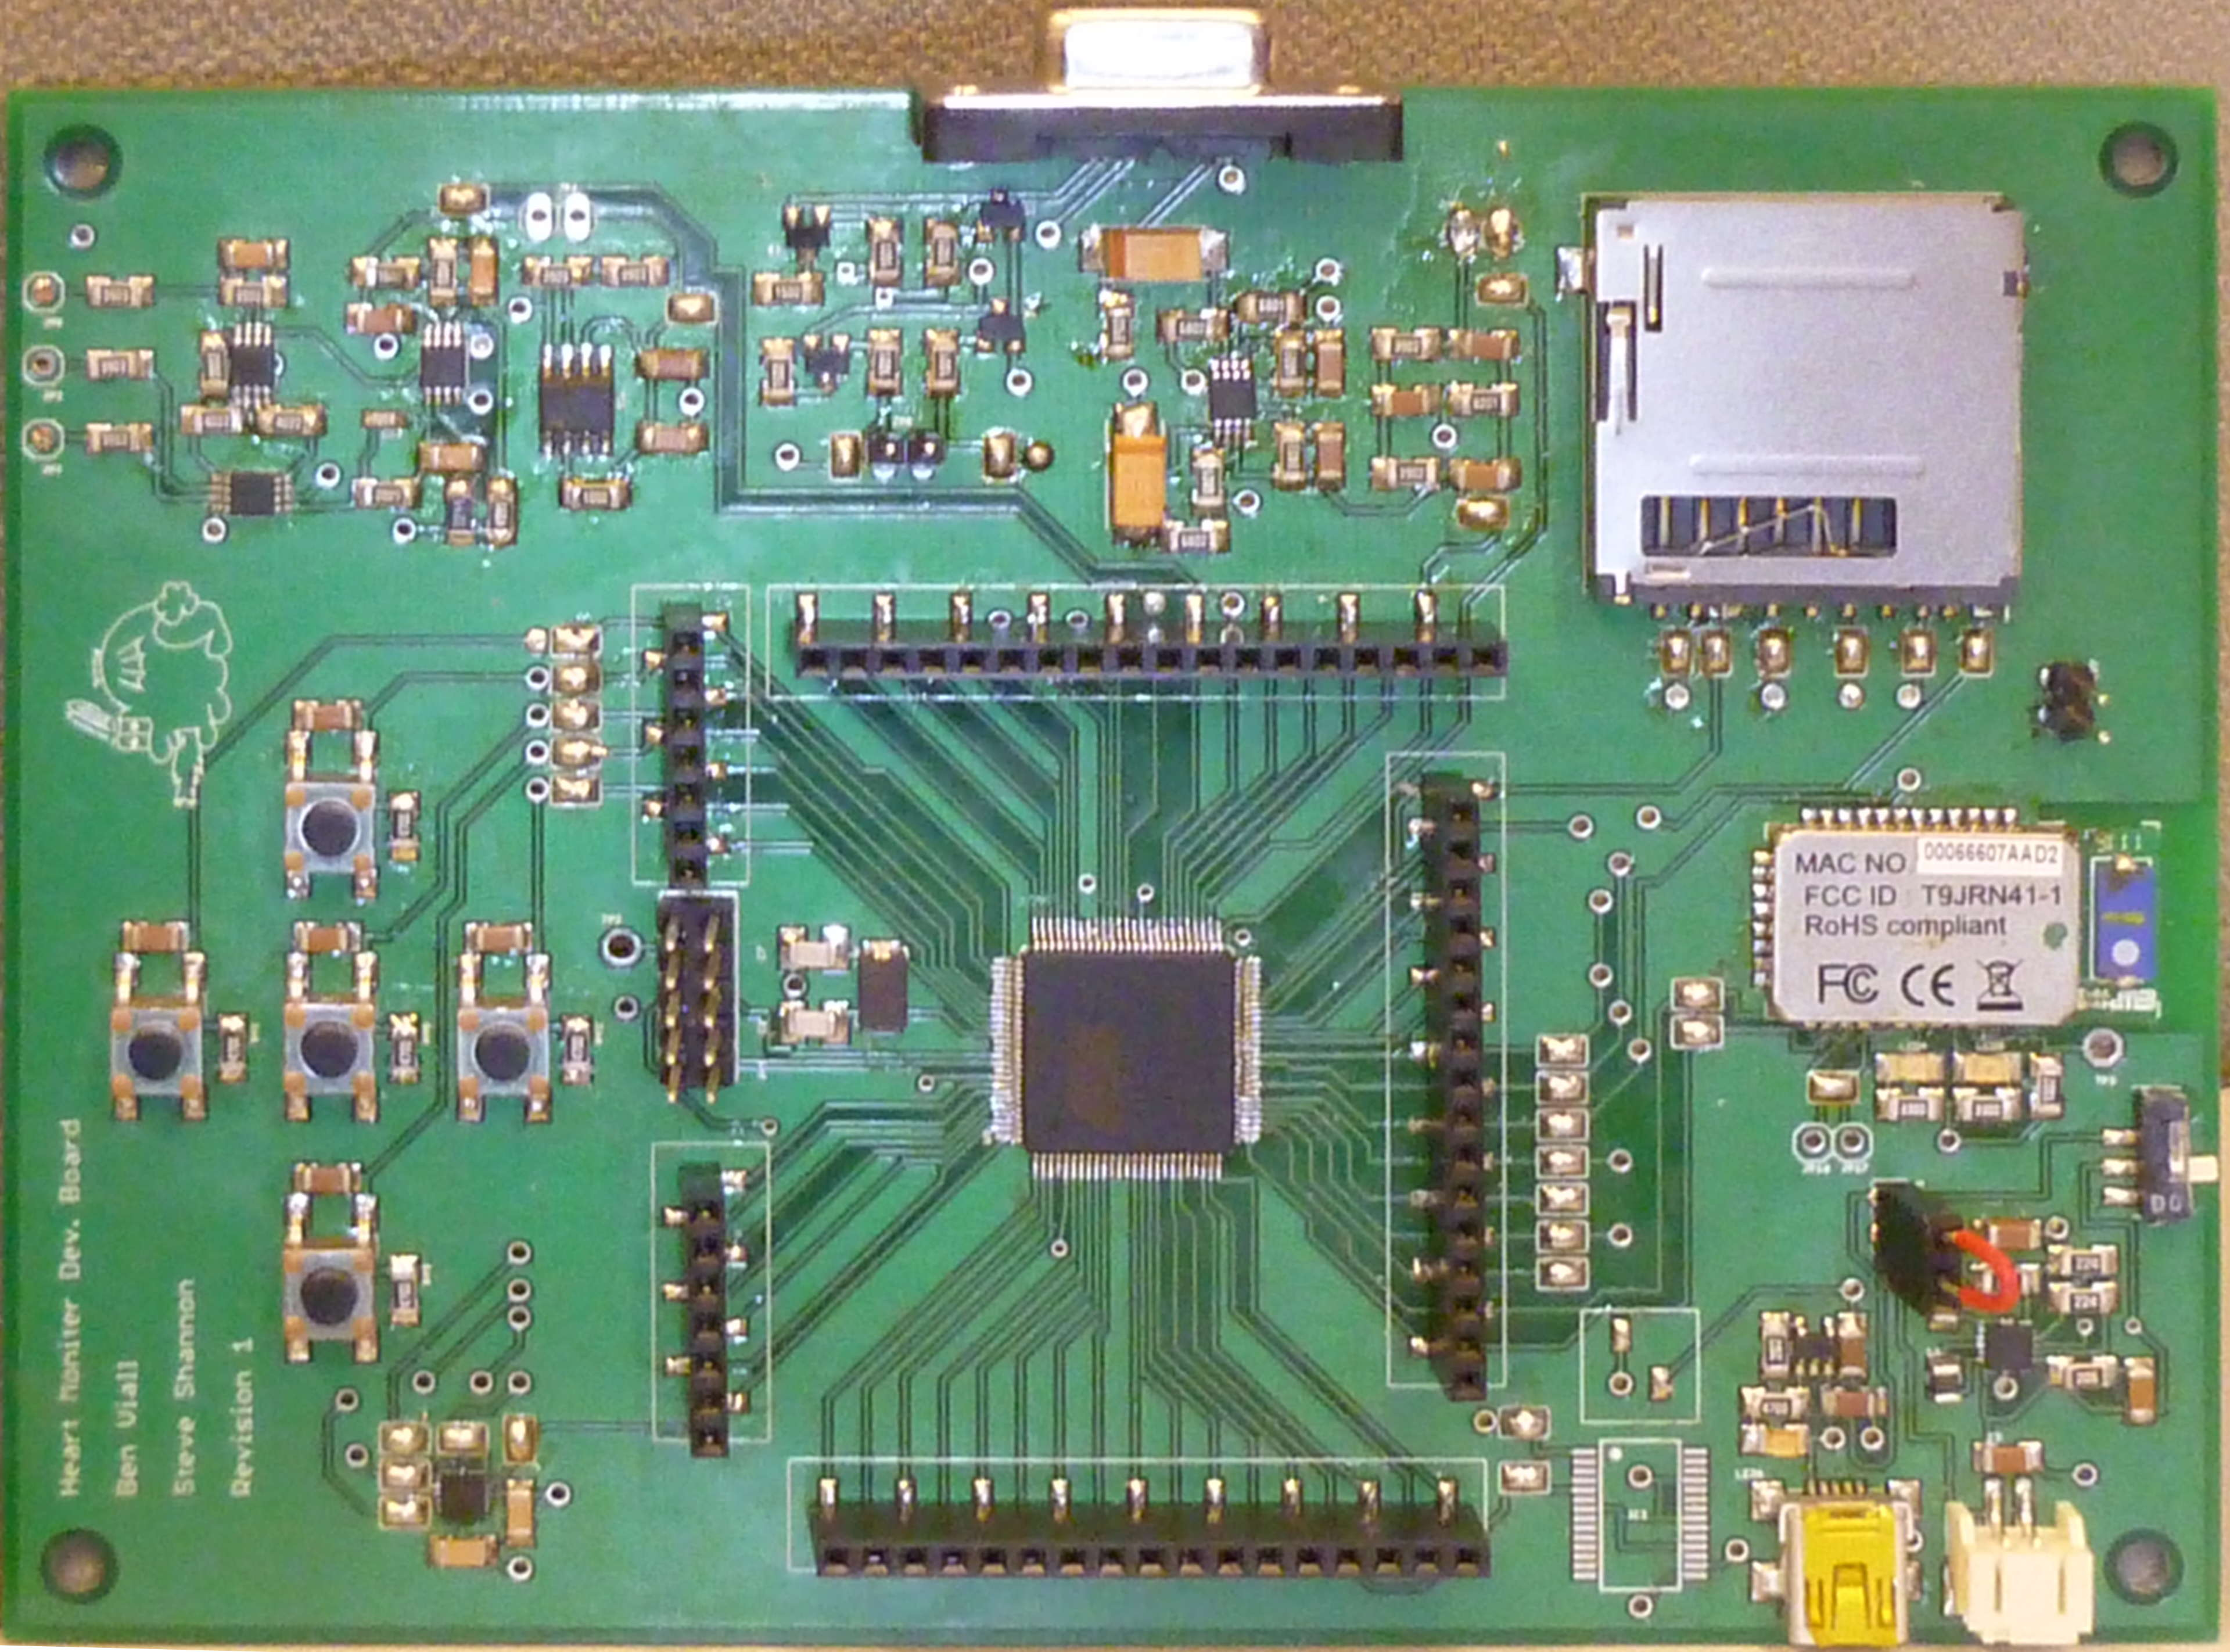
\includegraphics[scale=1,width=0.9\textwidth]{Images/PCB_Rev1.jpg} 
		\caption{MCHM PCB Rev 1}
	\end{center}
\end{figure}


Currently we are working on new designs for both ECG and \spo2 analog front-end (AFE) circuitry. These new designs will offload much of the filtering to software reducing components and cost. A Texas Instruments app note discusses trade-offs concerning AFE complexity and ADC design. [55] They present two scenarios for ECG signal acquisition. First, a 16-bit or lower resolution is presented. Preparing a signal for capture by a 16-bit ADC involves a significant amount of front end analog processing as show in \cref{fig:SAR_topology}.\cite{Soundarapandian2010} At each stage of the AFE, additional noise is inserted into the system. Furthermore, the complexity of the AFE design can significantly drive up cost.

\begin{figure}
	\begin{center}
		\label{fig:PCB_Rev3}
		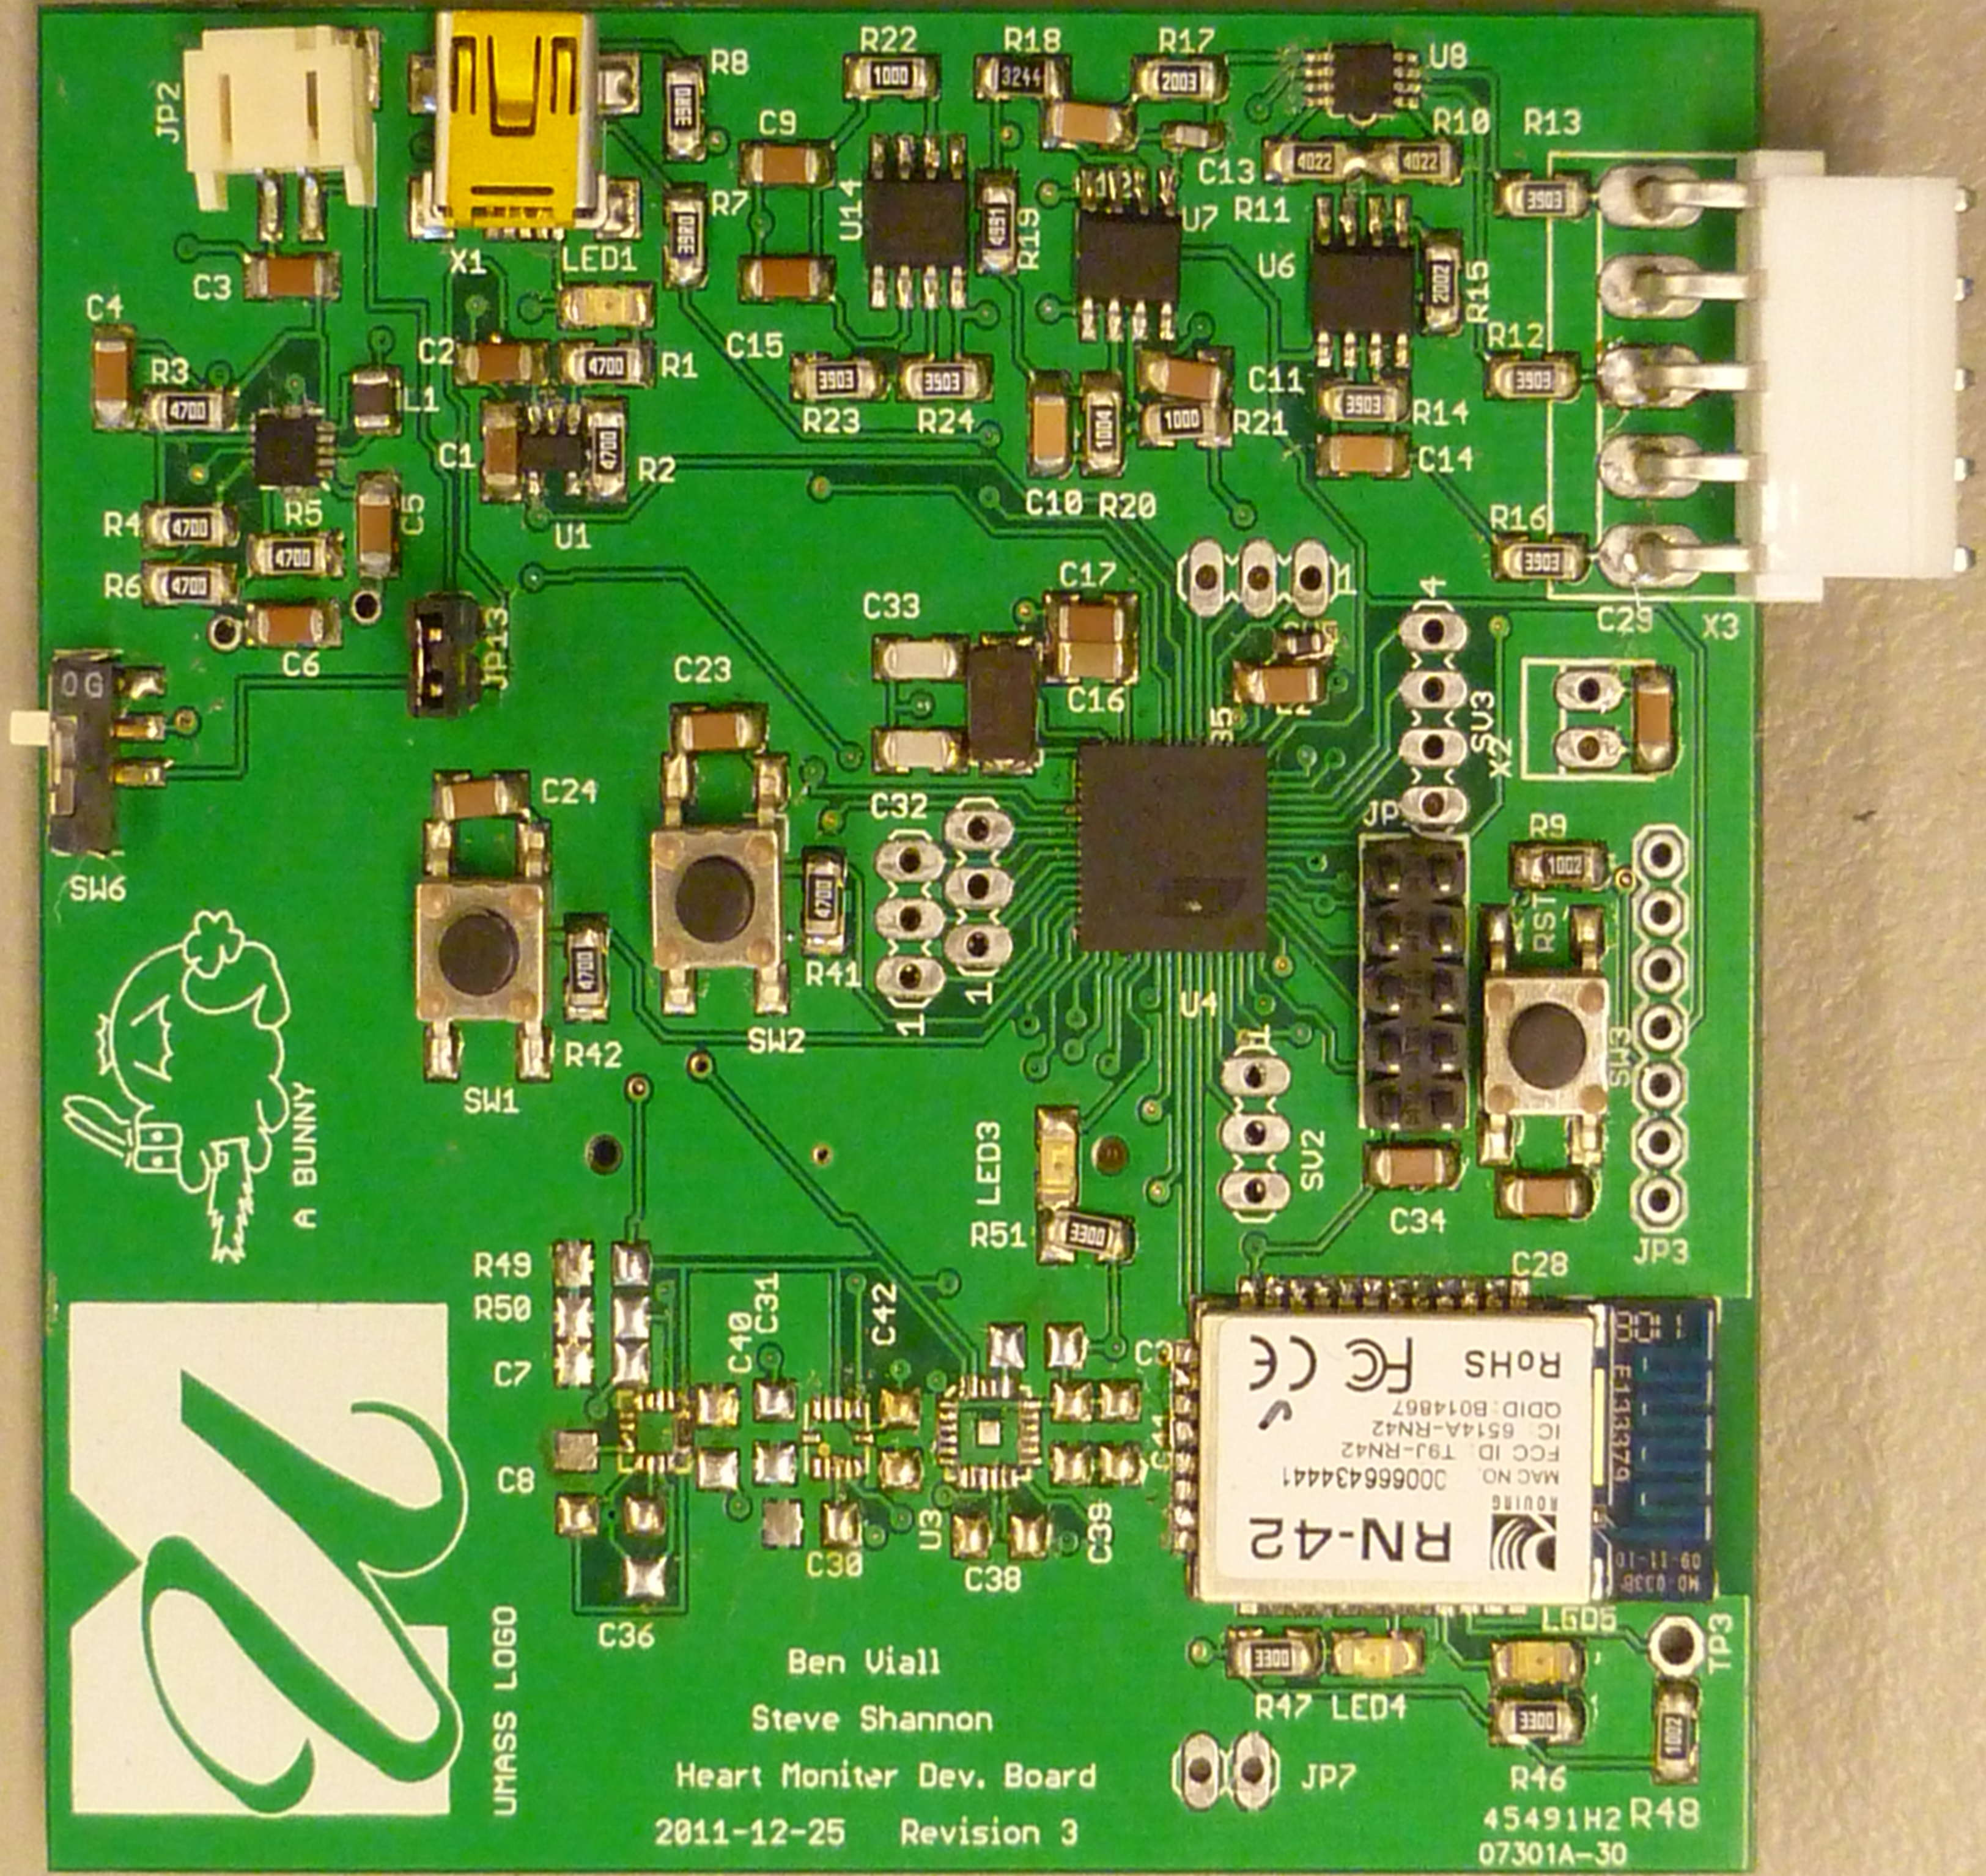
\includegraphics[scale=1,width=0.9\textwidth]{Images/PCB_Rev3.jpg} 
		\caption{MCHM PCB Rev 3}
	\end{center}
\end{figure}

However, the application note presents an alternative, shown in \cref{fig:sigmaDelta_topology}. \cite{Soundarapandian2010} Given a 24-bit sigma-delta ADC, only a low gain instrumentation amplifier and first order passive filter are needed to prepare the signal for conversion.  This approach offers higher accuracy than traditional ECG techniques and keeps the baseline drift of the signal intact allowing for more flexibility in the digital signal processing. We are currently designing an AFE component to capture both the ECG and \spo2 readings using the a $ \Sigma\Delta $ approach. Using the $ \Sigma\Delta $ approach simplifies future design problems. Designs can now have a simplified AFE and biometric signals can be filtered using simple to implement software filters using any hardware description language such as VHDL. This outcome is preferable to a fixed hardware design since it will allow more flexibility in the design stages. Adding additional features and filters need not increase hardware costs.


\begin{figure}
	\begin{center}
		\label{fig:SAR_topology}
		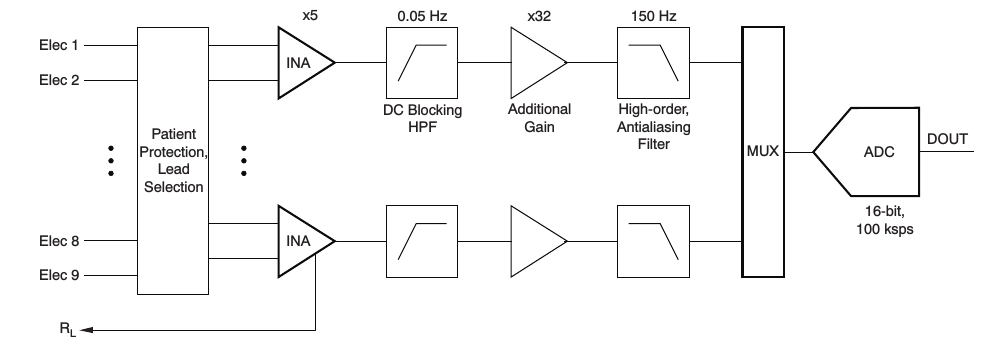
\includegraphics[scale=1,width=0.9\textwidth]{Images/SAR_topology.png} 
		\caption{Typical ECG acquisition system }
	\end{center}
\end{figure}

Other group research will be used as input to the dissertation. Previous, completed, master level research by Parma Chaiyasucheeva provided an elementary classification algorithm based on cardiac metrics\cite{Chaiyasucheeva2012}. Steven Shannon completed a master level thesis relating to fusing accelerometer data with other metrics and classifiers to combat movement artifacts\cite{Shannon2012}. Brendan Putin completed a master level project by creating a smartphone application to deliver psychosocial instruments and store the results in a database [TODO: find citation of putin]. Current work is being performed under my supervision by master level candidates. Patrick DaSilva is working to classify ECG signals based on their components and continue Parma Chaiyasucheeva's work on patient wellness calculation. Alexander Ekholm is researching PPG sensor technologies. Specifically, design, implementation, and validation of a sensor capable of reflective PPG collection at a non-peripheral site, near the heart.  Also, under development, Brian Lauro is working on a minimal cardiac ontology, and BKE.

\begin{figure}
	\begin{center}
		\label{fig:sigmaDelta_topology}
		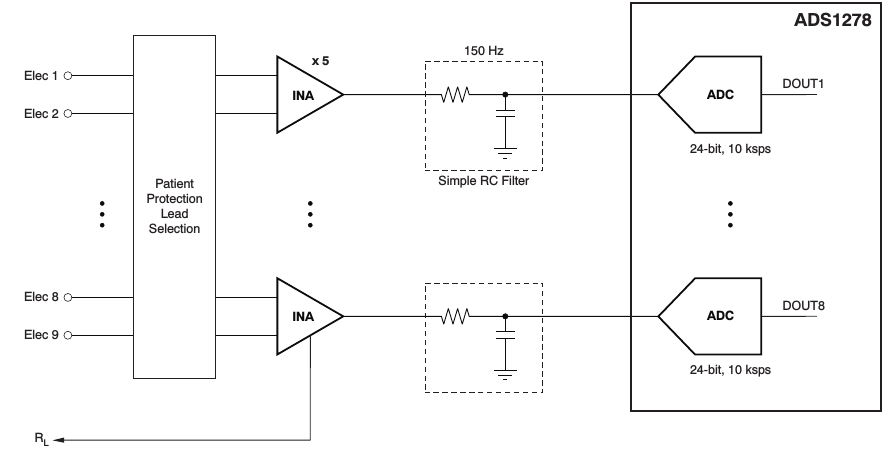
\includegraphics[scale=1,width=0.9\textwidth]{Images/sigmaDelta_topology_simultanious.png} 
		\caption{ECG approach using $\Sigma\Delta $ ADC}
	\end{center}
\end{figure}

\section{Description of Dissertation Chapters}
\iffalse
\subsection{\Cref{chap:introduction} introduction}
\label{subsec:Chapter1Introduction}
In the Introduction chapter, I will discuss the current state of medical care for CHF patients. I will present the relevant statistics about hospitalization and mortality. I will then cover the topic of engaging patients in their own self-care, citing relevant studies and statistics. Then finally indicate my proposed solution.
\subsection{\Cref{chap:LitReview} Literature review}
\label{subsec:Chapter2LitReview}
This section will first cover previous research done in the fields of ECG, \spo2 /PPG, and acceleration sensors. Then a discussion of how to derive synthetic sensor measurements based on acquired ECG, \spo2 /PPG, and acceleration measurements. I will focus on literature with methods of deriving heart rate, blood pressure without an inflatable cuff, and deriving respiration rate without a chest strap. Next, I will present methods for removing noise from the ECG and PPG sensors based on accelerometer data. Finally, the pertinent literature in the medical domain will be reviewed, paying specific attention to the fields of patient education and self-care as well as the psychosocial instruments to be used, the MLHF, DASI, and HFSA.

\subsection{\Cref{chap:SysDesign} System Design Concepts}
\label{subsec:Chapter3SystemDesignConcepts}
In this chapter, I will detail the design decisions encountered while implementing the WHIPPED end-to-end system. I will discuss concepts in three sections: the sensor suite, the smartphone app, and the BKE.

\subsection{\Cref{chap:SensorConcepts} Sensor concepts}
\label{subsec:Chapter4SensorConcepts}
In this chapter, I will cover in detail the code and DSP techniques used in the data flow of the sensor designs covering both the analog front end for the real sensors and the software DSP and data fusion techniques for the synthetic sensors.

\subsection{ Hardware designs}
\label{subsec:Chapter5HardwareDesigns}
In this chapter, I will address various hardware decisions I encountered while designing the senor suite and its communication with the smartphone app. I will also address power usage of the device and any layout related board issues. Finally, I will address the packaging of the device into a wearable sensor.

\subsection{\Cref{chap:ProtoTypeBuildTest} Integration and Testing}
\label{subsec:Chapter6IntegrationAndTesting}
This chapter will detail the process of integrating the three parts of the WHIPPED system together to make an end-to-end application. I will first discuss integrating the smartphone and sensor suite to gather physiometric data. Then discuss the integration of the smartphone and BKE, separate from the sensors, to communicate psychosocial information. Finally, I will discuss the BKE‘s integration of all knowledge from both the sensors, via the smartphone, and the psychosocial data to calculate wellness and provide interventions.
%
%\subsection{Chapter 7. Data mining/cardiac ontology}
%\label{subsec:Chapter7DataMining}
%After implementing the WHIPPED system, validation will be performed in two steps. First, basic validation and safety will be performed on healthy, %volunteer members of the research group (who have IRB approval). Then, an experimental nursing study consisting of volunteer CHF patients, who have %received informed consent in accordance with IRB rules.

\subsection{Chapter 8. Conclusions/ Future work}
\label{subsec:Chapter8Conclusions}
Validating my system with an exploratory study is only the first step in a larger design philosophy. I will indicate avenues of improvement for hardware and software focusing on moving to a system on a chip (SoC) design. I will present my conclusions and suggest future steps in the research.

\fi
